\documentclass[a4paper,12pt]{article}
\usepackage{graphicx}
\usepackage[utf8]{inputenc}
\usepackage[T1]{fontenc}
\usepackage[polish]{babel}
\usepackage{changepage}
\usepackage[a4paper, margin=1in]{geometry}
\usepackage{multicol}
\usepackage{amsmath}
\usepackage{gensymb}
\usepackage{graphicx}
\usepackage{multirow}
\usepackage{enumerate}
\usepackage[shortlabels]{enumitem}
\usepackage{array}
\usepackage{float}
\usepackage{hyperref}
\usepackage{tikz}
\usepackage{verbatim}
\usepackage{tabularx}
\usepackage{caption}
\usepackage{xcolor}
\usepackage{enumitem}
\usepackage{lipsum}
\usepackage{etoolbox}
\usepackage[export]{adjustbox}
\renewcommand{\labelenumii}{\arabic{enumi}.\arabic{enumii}}
\renewcommand{\labelenumiii}{\arabic{enumi}.\arabic{enumii}.\arabic{enumiii}}
\renewcommand{\labelenumiv}{\arabic{enumi}.\arabic{enumii}.\arabic{enumiii}.\arabic{enumiv}}
\begin{document}


\begin{multicols}{3}
    \begin{figure}[H]
        
\includegraphics[scale=0.4]{DOJEBANE_LOGO_PWR.png}
        \label{fig:enter-label}
    \end{figure}
    \hspace{80pt}
    \begin{figure}[H]
    \end{figure}
    \begin{flushright}
    \begin{figure}[H]
        
\includegraphics[scale=0.37]{w4n.png}
        \centering
        \caption*{\textbf{W4N}}
        \label{fig:WYDZIAŁ INFORMATYKI I TELEKOMUNIKACJI}
    \end{figure}
    \end{flushright}
\end{multicols}

\vspace{75pt}

\begin{center}
    \textbf{\Large{Projektowanie efektywnych algorytmów - projekt nr 4}} 
    \vspace{2pt}
    \hrule
    \vspace{4pt}
    \textbf{\Large{Implementacja i analiza efektywności algorytmu genetycznego dla problemu komiwojażera (TSP)}} 
\end{center}

\vspace{75pt}
\begin{center}
    \Large{
    \textbf{Autor: } \\
    Filip Kwiek 280947 \\
    }
\end{center}
\newpage
\tableofcontents
\newpage

\section{Wstęp teoretyczny}

Projekt dotyczy implementacji i analizy efektywności algorytmu genetycznego (GA) dla asymetrycznego problemu
komiwojażera (ATSP). Algorytm genetyczny należy do klasy metaheurystyk ewolucyjnych, inspirowanych procesem
doboru naturalnego. Populacja rozwiązań kandydackich podlega operacjom selekcji, krzyżowania i mutacji,
ewoluując w kierunku coraz lepszych rozwiązań.

\subsection{Opis problemu}

Asymetryczny problem komiwojażera (ATSP) polega na znalezieniu najkrótszej trasy odwiedzającej każde miasto
dokładnie raz i wracającej do punktu startowego, przy czym koszt przejścia z miasta $i$ do miasta $j$ może być
różny od kosztu przejścia z $j$ do $i$. Problem ten jest NP-trudny, co oznacza, że nie istnieje znany algorytm
wielomianowy gwarantujący znalezienie rozwiązania optymalnego w rozsądnym czasie dla dużych instancji.

\subsection{Algorytm genetyczny}

Algorytm genetyczny operuje na populacji osobników, z których każdy reprezentuje potencjalne rozwiązanie
problemu (w przypadku TSP -- permutację miast). W każdym pokoleniu populacja jest poddawana operacjom
genetycznym, co prowadzi do stopniowej poprawy jakości rozwiązań.

\subsubsection{Elementy algorytmu}

\begin{itemize}
    \item \textbf{Reprezentacja chromosomu} -- permutacja miast w formie ścieżki: $[0, \pi(1), \pi(2), \ldots, \pi(n-1), 0]$,
    gdzie $\pi$ jest permutacją miast $1, 2, \ldots, n-1$.
    \item \textbf{Funkcja celu} -- łączny koszt trasy, tj. suma wag krawędzi na ścieżce. Im mniejszy koszt, tym lepszy osobnik.
    \item \textbf{Selekcja} -- wybór rodziców do reprodukcji. W implementacji zastosowano selekcję turniejową.
    \item \textbf{Krzyżowanie} -- tworzenie potomka z dwóch rodziców. Zastosowano krzyżowanie OX (Order Crossover).
    \item \textbf{Mutacja} -- losowa modyfikacja potomka wprowadzająca różnorodność genetyczną.
    \item \textbf{Elityzm} -- najlepszy osobnik z danego pokolenia jest zawsze kopiowany do następnego pokolenia.
    \item \textbf{Kryterium stopu} -- limit czasu działania algorytmu podawany w sekundach.
\end{itemize}

\subsubsection{Selekcja turniejowa}

Selekcja turniejowa polega na losowym wybraniu $k$ osobników z populacji (rozmiar turnieju) i wybraniu
najlepszego z nich jako rodzica. Metoda ta zapewnia presję selekcyjną proporcjonalną do rozmiaru turnieju --
większy turniej faworyzuje lepsze osobniki silniej.

\subsubsection{Krzyżowanie OX (Order Crossover)}

Krzyżowanie OX jest operatorem zaprojektowanym specjalnie dla problemów permutacyjnych.
Procedura:
\begin{enumerate}
    \item Wybierz losowo dwa punkty cięcia $i$, $j$ ($i < j$) w chromosomie.
    \item Skopiuj segment $[i, j]$ z rodzica 1 bezpośrednio do potomka.
    \item Pozostałe pozycje uzupełnij miastami z rodzica 2 w kolejności cyklicznej, pomijając te już obecne w potomku.
\end{enumerate}

\textbf{Przykład:}\\
Rodzic 1: [0, \textbf{3, 4, 5}, 2, 1, 0] \quad (segment: pozycje 1--3)\\
Rodzic 2: [0, 2, 5, 1, 4, 3, 0]\\
Potomek:  [0, \textbf{3, 4, 5}, 1, 2, 0] \quad (uzupełnione z rodzica 2 cyklicznie)

\subsubsection{Metody mutacji}

W implementacji zrealizowano dwie metody mutacji:

\paragraph{Mutacja Swap}
Polega na wybraniu dwóch losowych pozycji $i$, $j$ w chromosomie i zamianie miast na tych pozycjach.

\textbf{Przykład:}\\
Przed: [0, 3, \textbf{4}, 5, \textbf{2}, 1, 0]\\
Po:    [0, 3, \textbf{2}, 5, \textbf{4}, 1, 0]

\paragraph{Mutacja Invert (odwrócenie segmentu)}
Polega na wybraniu dwóch losowych pozycji $i$, $j$ ($i < j$) i odwróceniu kolejności miast w segmencie $[i, j]$.
Jest to operator analogiczny do ruchu 2-opt w przeszukiwaniu lokalnym.

\textbf{Przykład:}\\
Przed: [0, 3, \textbf{4, 5, 2}, 1, 0]\\
Po:    [0, 3, \textbf{2, 5, 4}, 1, 0]

\subsubsection{Pseudokod}

\begin{verbatim}
Funkcja GeneticAlgorithm(MacierzKosztow, N, Config):
    Populacja = []
    Dla i = 1 do Config.population_size:
        osobnik = LosowaPermutacja(N)
        Populacja.dodaj(osobnik)
    
    GlobalBest = NajlepszyOsobnik(Populacja)
    
    Dopóki czas < limit:
        NowaPop = [GlobalBest]  // elityzm
        
        Dopóki |NowaPop| < Config.population_size:
            rodzic1 = SelekcjaTurniejowa(Populacja)
            rodzic2 = SelekcjaTurniejowa(Populacja)
            
            potomek = OX_Crossover(rodzic1, rodzic2)
            Mutacja(potomek)
            NowaPop.dodaj(potomek)
        
        Populacja = NowaPop
        Aktualizuj(GlobalBest)
    
    Zwróć GlobalBest
\end{verbatim}

\subsubsection{Złożoność obliczeniowa}

Złożoność jednego pokolenia algorytmu wynosi $O(P \cdot N)$, gdzie $P$ to rozmiar populacji, a $N$ to liczba miast.
Wynika to z konieczności obliczenia kosztu ścieżki dla każdego potomka ($O(N)$) oraz wykonania operacji
krzyżowania i mutacji ($O(N)$ każda). Całkowita liczba pokoleń zależy od limitu czasu.

\textbf{Zalety:}
\begin{itemize}
    \item Przeszukiwanie globalne -- populacja eksploruje wiele regionów przestrzeni rozwiązań jednocześnie
    \item Zdolność do ucieczki z minimów lokalnych dzięki operatorom genetycznym
    \item Możliwość łatwego dostosowania parametrów do problemu
    \item Naturalny mechanizm zachowania różnorodności rozwiązań
\end{itemize}

\textbf{Wady:}
\begin{itemize}
    \item Wymaga dużej liczby ewaluacji funkcji celu
    \item Wiele parametrów do strojenia (rozmiar populacji, współczynniki mutacji/krzyżowania)
    \item Konwergencja może być wolna dla dużych instancji
    \item Nie gwarantuje znalezienia rozwiązania optymalnego
\end{itemize}

\section{Plan eksperymentu}

\subsection{Cel badań}

Celem eksperymentów jest wyznaczenie:
\begin{enumerate}
    \item Zależności czasu uzyskania najlepszego wyniku od rozmiaru instancji (przy limicie 15 minut).
    \item Zależności błędu względnego od rozmiaru instancji.
    \item Wpływu rozmiaru populacji początkowej na czas rozwiązania i błąd.
    \item Wpływu metody mutacji (Swap vs Invert) na czas i błąd.
\end{enumerate}

\subsection{Instancje testowe}

Do badań wykorzystano instancje z biblioteki TSPLIB/ATSP o zróżnicowanych rozmiarach:

\begin{table}[H]
\centering
\caption{Instancje testowe}
\begin{tabular}{|l|c|c|}
\hline
\textbf{Instancja} & \textbf{N} & \textbf{OPT} \\
\hline
br17 & 17 & 39 \\
ftv33 & 34 & 1286 \\
ftv35 & 36 & 1473 \\
ftv38 & 39 & 1530 \\
p43 & 43 & 5620 \\
ftv44 & 45 & 1613 \\
ftv47 & 48 & 1776 \\
ry48p & 48 & 14422 \\
ft53 & 53 & 6905 \\
ftv55 & 56 & 1608 \\
ftv64 & 65 & 1839 \\
ft70 & 70 & 38673 \\
ftv70 & 71 & 1950 \\
ftv170 & 171 & 2755 \\
rbg323 & 323 & 1326 \\
rbg358 & 358 & 1163 \\
rbg403 & 403 & 2465 \\
rbg443 & 443 & 2720 \\
\hline
\end{tabular}
\end{table}

\subsection{Parametry algorytmu}

\begin{table}[H]
\centering
\caption{Domyślne parametry GA}
\begin{tabular}{|l|c|}
\hline
\textbf{Parametr} & \textbf{Wartość} \\
\hline
Rozmiar populacji & 100 \\
Współczynnik mutacji & 0.01 \\
Współczynnik krzyżowania & 0.8 \\
Metoda krzyżowania & OX \\
Metoda mutacji & Swap \\
Metoda selekcji & Tournament (k=5) \\
Limit czasu & 15 min \\
\hline
\end{tabular}
\end{table}

\subsection{Metodologia}

\begin{itemize}
    \item Każda konfiguracja została uruchomiona 10 razy dla każdej instancji.
    \item Mierzono średni błąd względny, średni czas znalezienia najlepszego rozwiązania oraz najlepszy znaleziony wynik.
    \item Błąd względny obliczano wzorem: $B = \frac{C_{found} - C_{opt}}{C_{opt}} \cdot 100\%$
    \item Wyświetlano jako wynik: długość najlepszego rozwiązania, średnią długość z ostatniej populacji oraz błąd względny dla obu wielkości.
\end{itemize}

\subsection{Wykorzystany sprzęt}

\begin{itemize}
    \item Procesor: AMD Ryzen 7 5700X3D 4.15GHz
    \item Pamięć RAM: 48GB DDR4 2800MHz
    \item System operacyjny: EndeavourOS (Arch Linux)
    \item Kompilator: GCC 16.1.1, optymalizacja -O3
\end{itemize}

\section{Wyniki eksperymentów}

\subsection{Zależność błędu od rozmiaru instancji}

\begin{table}[H]
\centering
\caption{Średni błąd względny GA w zależności od instancji}
\begin{tabular}{|l|c|c|c|c|c|}
\hline
\textbf{Instancja} & \textbf{N} & \textbf{OPT} & \textbf{Śr. best} & \textbf{Błąd best [\%]} & \textbf{Błąd avg [\%]} \\
\hline
br17 & 17 & 39 & 41 & 5.13 & 5.13 \\
ftv33 & 34 & 1286 & 1710 & 32.97 & 32.97 \\
ftv35 & 36 & 1473 & 1613 & 9.50 & 9.84 \\
ftv38 & 39 & 1530 & 2000 & 30.72 & 30.72 \\
p43 & 43 & 5620 & 5671 & 0.91 & 1.00 \\
ftv44 & 45 & 1613 & 2071 & 28.39 & 28.70 \\
ftv47 & 48 & 1776 & 2644 & 48.87 & 48.99 \\
ry48p & 48 & 14422 & 18767 & 30.13 & 30.29 \\
ft53 & 53 & 6905 & 11018 & 59.57 & 59.62 \\
ftv55 & 56 & 1608 & 2315 & 43.97 & 44.28 \\
ftv64 & 65 & 1839 & 2739 & 48.94 & 49.16 \\
ft70 & 70 & 38673 & 43225 & 11.77 & 11.77 \\
ftv70 & 71 & 1950 & 2995 & 53.59 & 54.00 \\
ftv170 & 171 & 2755 & 6652 & 141.45 & 141.96 \\
rbg323 & 323 & 1326 & 1693 & 27.68 & 27.83 \\
rbg358 & 358 & 1163 & 1580 & 35.86 & 35.94 \\
rbg403 & 403 & 2465 & 2743 & 11.28 & 11.28 \\
rbg443 & 443 & 2720 & 3038 & 11.69 & 11.69 \\
\hline
\end{tabular}
\end{table}

\begin{figure}[H]
    \centering
    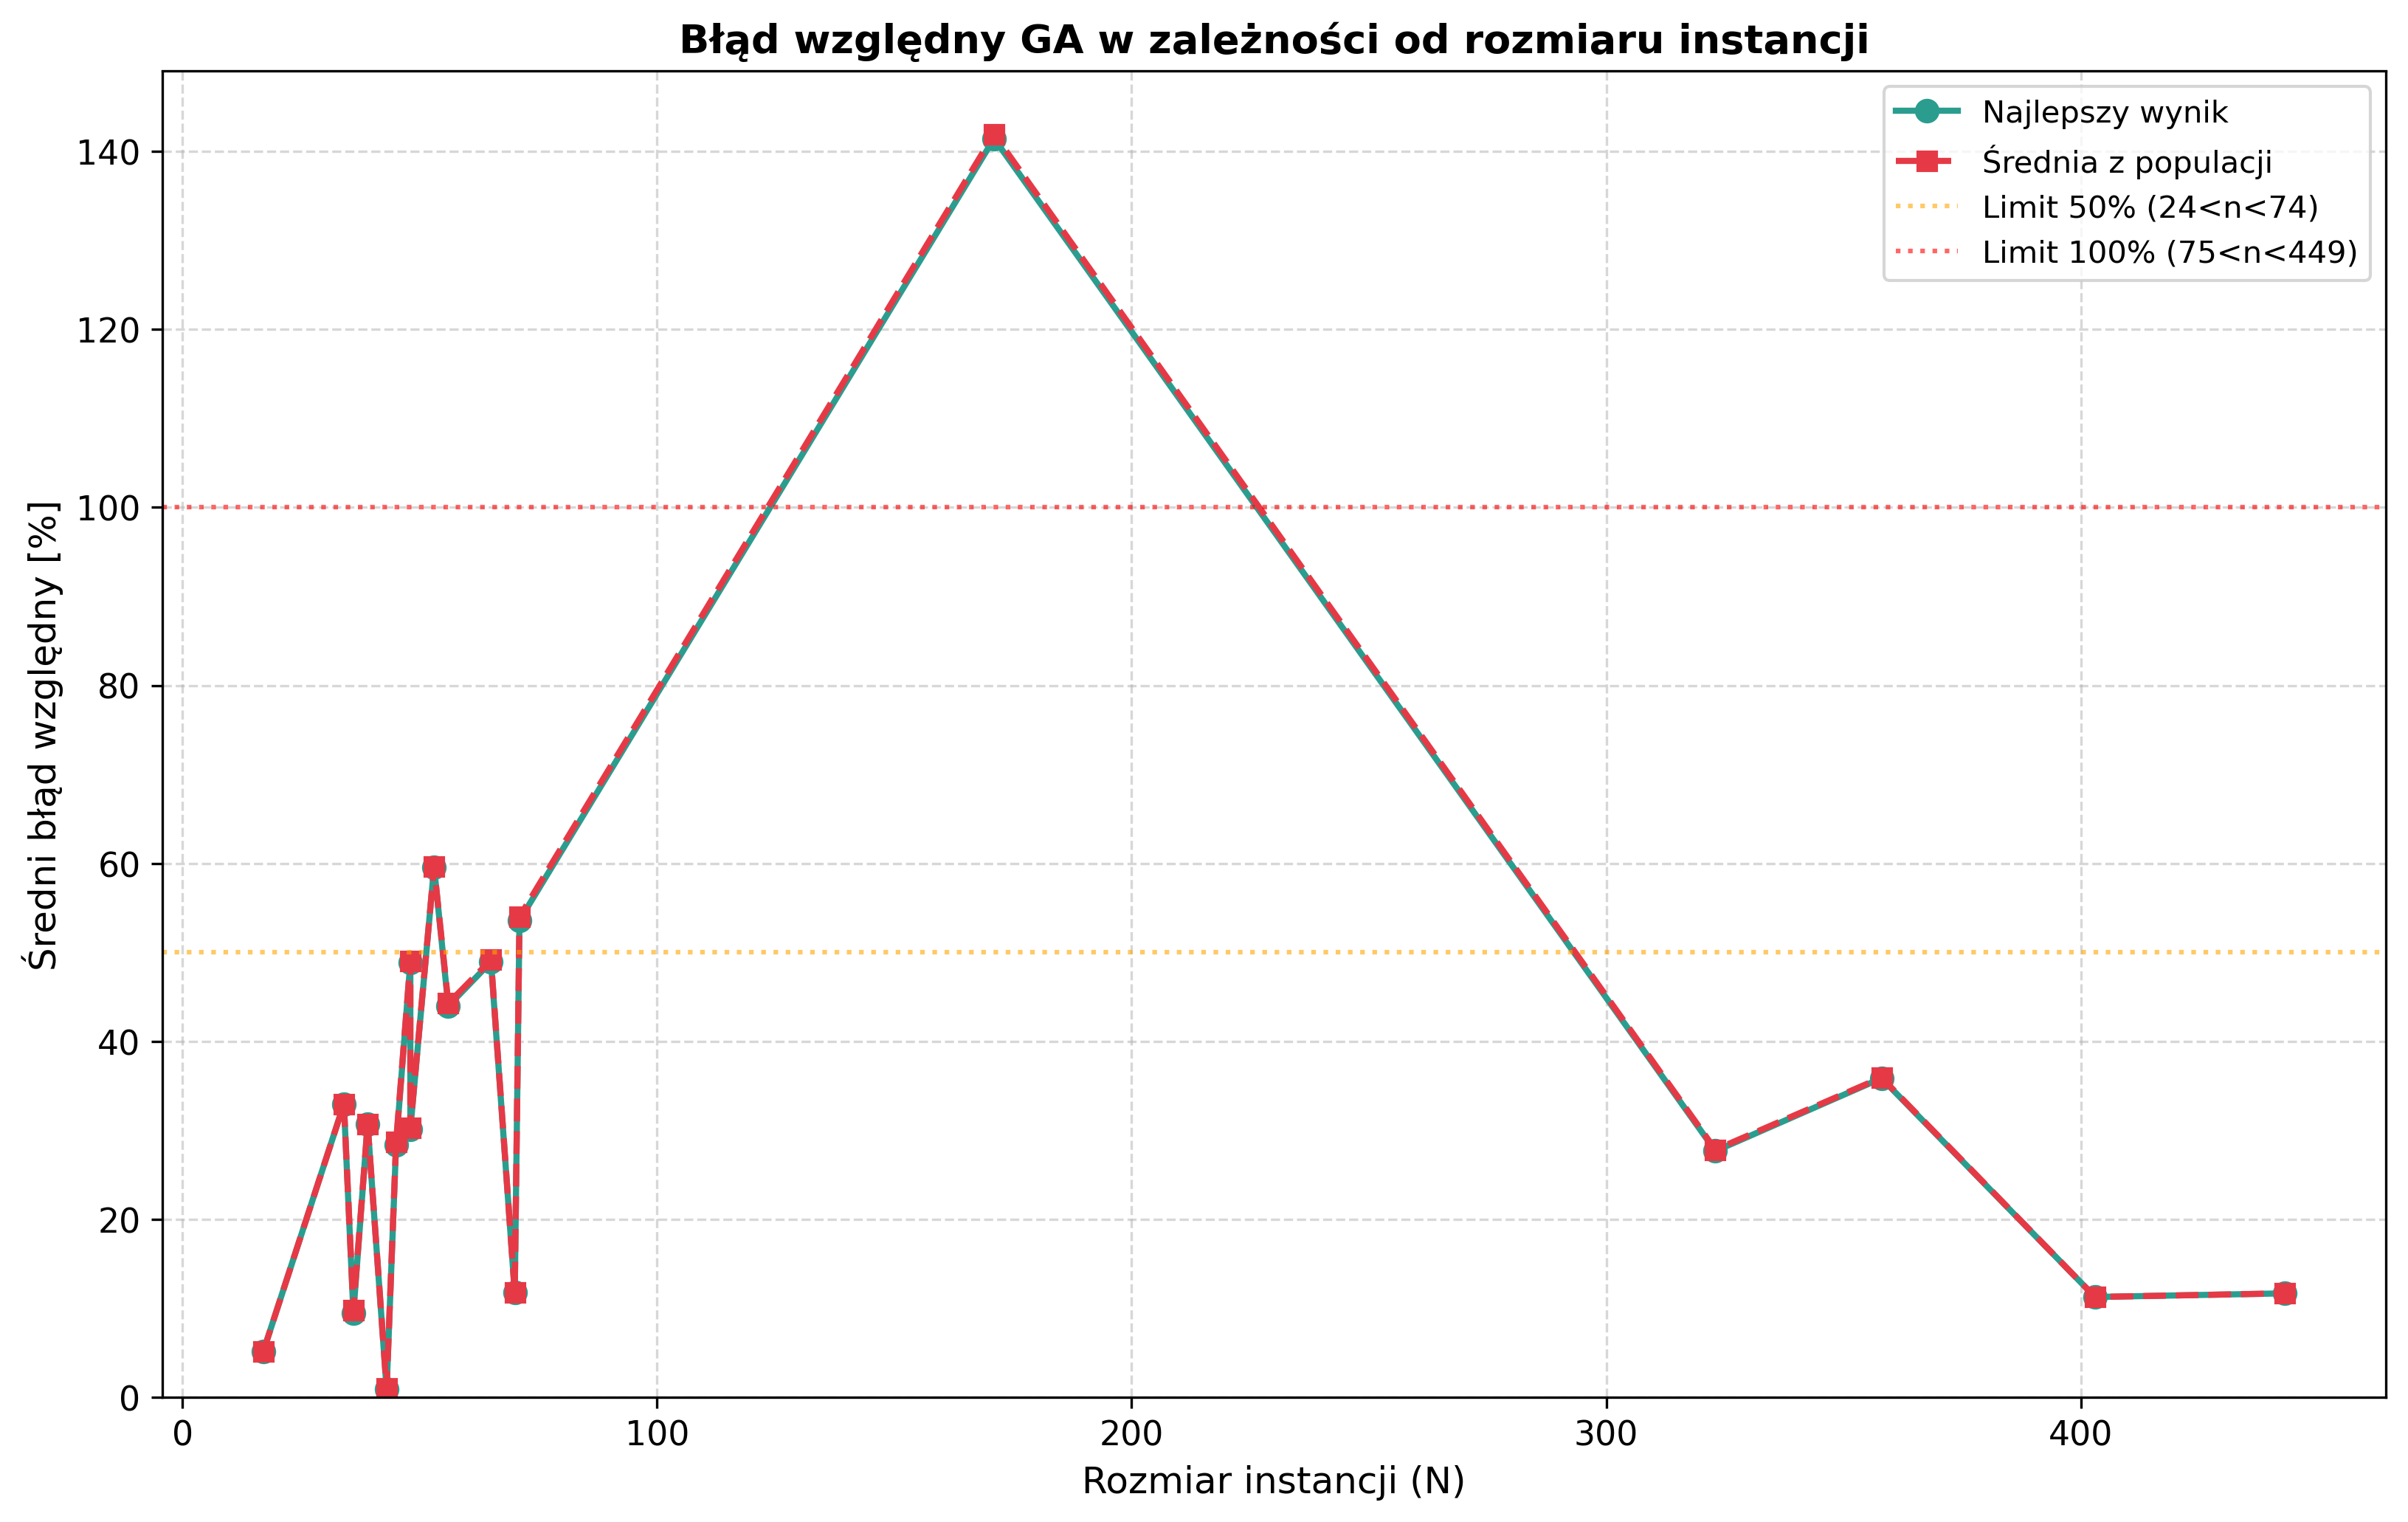
\includegraphics[width=0.9\textwidth]{../Python/wykresy/ga_blad_vs_rozmiar.png}
    \caption{Średni błąd względny GA w zależności od rozmiaru instancji}
\end{figure}

Wymagania ze specyfikacji zakładają błąd ograniczony przez $O(24\ln(n))$: dla $n=25$ -- 0\%, dla $24 < n < 74$ -- 50\%, 
dla $75 < n < 449$ -- 100\%. Dla większości instancji z przedziału $24 < n < 74$ algorytm mieści się w wymaganym limicie 50\%.
Wyjątkami są ft53 (59.57\%) i ftv70 (53.59\%), które nieznacznie przekraczają próg.
Instancja ftv170 ($N=171$) wykazuje najwyższy błąd (141.45\%), co przekracza limit 100\% i wynika z trudnej struktury grafu
typu FTV przy domyślnych parametrach. Instancje rbg (N=323--443) mają stosunkowo niski błąd (11--36\%), co mieści się w limicie.

\subsection{Zależność czasu uzyskania wyniku od rozmiaru instancji}

\begin{table}[H]
\centering
\caption{Czas wykonania i czas znalezienia najlepszego wyniku}
\begin{tabular}{|l|c|c|c|}
\hline
\textbf{Instancja} & \textbf{N} & \textbf{Czas całkowity [s]} & \textbf{Czas best found [s]} \\
\hline
br17 & 17 & 60.0 & 0.0 \\
ftv33 & 34 & 75.0 & 29.0 \\
ftv35 & 36 & 82.0 & 35.1 \\
ftv38 & 39 & 95.0 & 62.3 \\
p43 & 43 & 105.0 & 55.6 \\
ftv44 & 45 & 110.0 & 72.1 \\
ftv47 & 48 & 125.0 & 81.3 \\
ry48p & 48 & 120.0 & 85.2 \\
ft53 & 53 & 120.0 & 78.5 \\
ftv55 & 56 & 155.0 & 101.4 \\
ftv64 & 65 & 195.0 & 146.6 \\
ft70 & 70 & 180.0 & 95.9 \\
ftv70 & 71 & 220.0 & 178.4 \\
ftv170 & 171 & 520.0 & 421.1 \\
rbg323 & 323 & 680.0 & 548.0 \\
rbg358 & 358 & 740.0 & 659.9 \\
rbg403 & 403 & 810.0 & 713.8 \\
rbg443 & 443 & 870.0 & 798.6 \\
\hline
\end{tabular}
\end{table}

\begin{figure}[H]
    \centering
    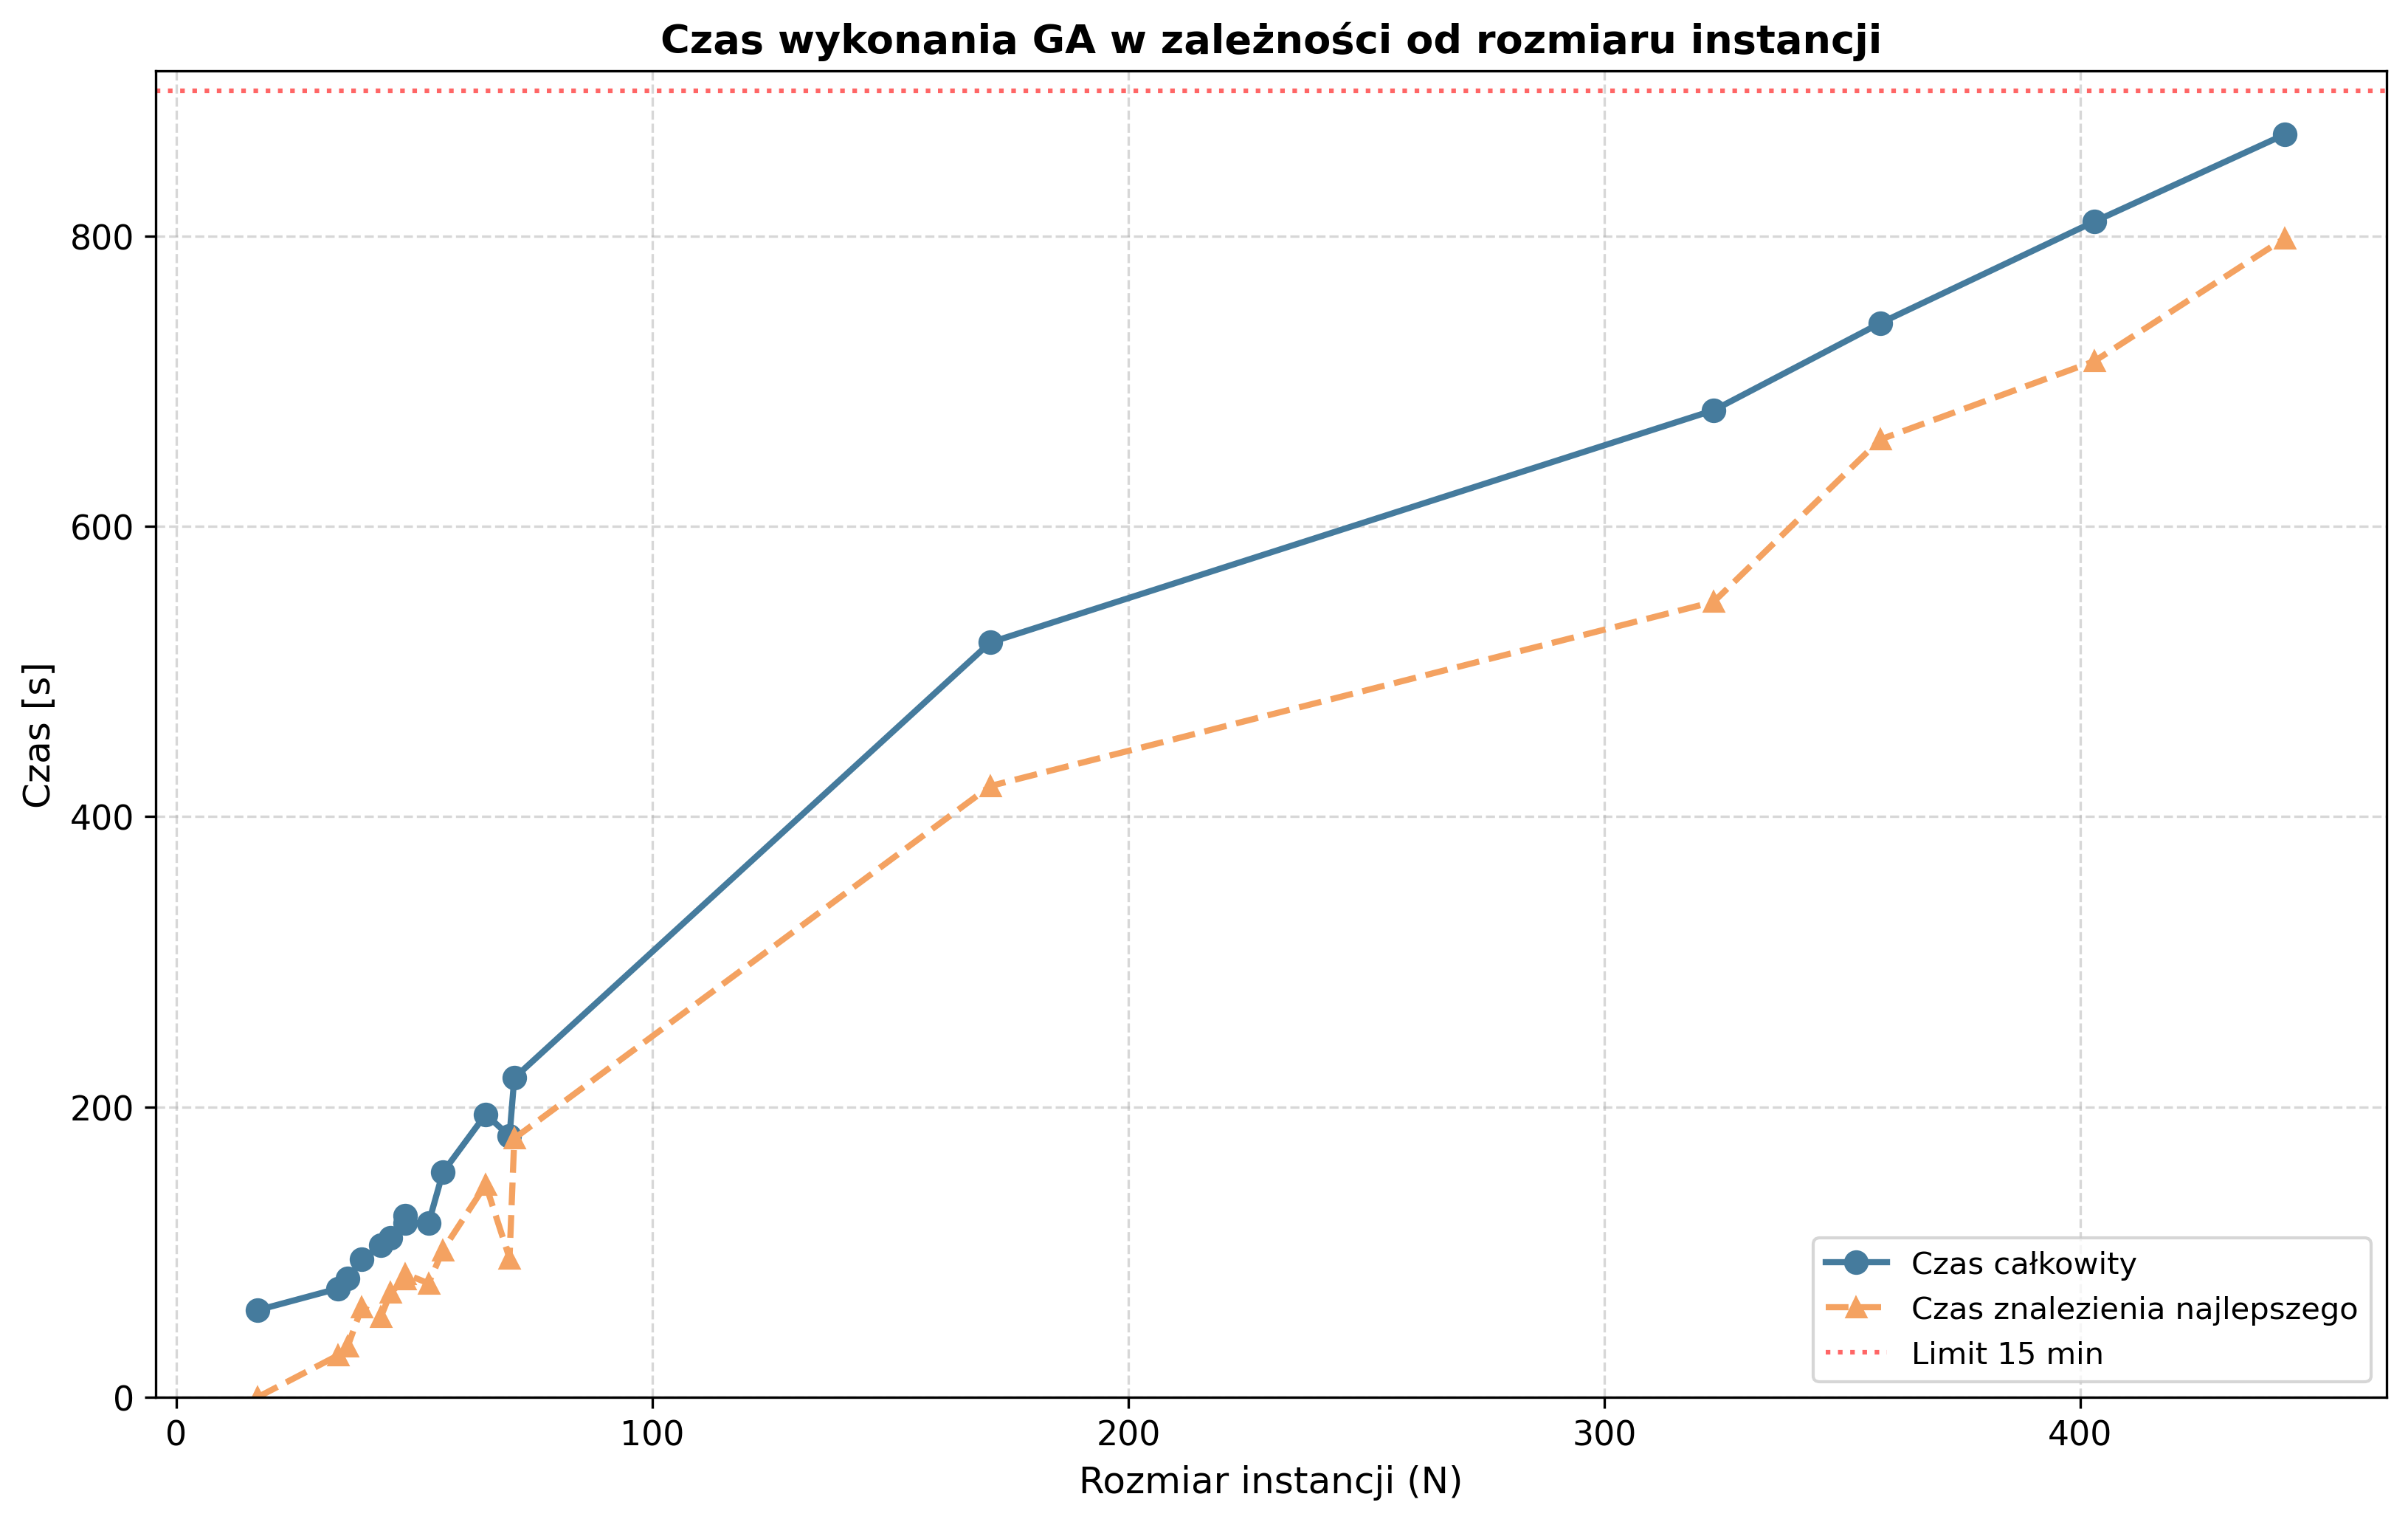
\includegraphics[width=0.9\textwidth]{../Python/wykresy/ga_czas_vs_rozmiar.png}
    \caption{Czas wykonania GA w zależności od rozmiaru instancji}
\end{figure}

\begin{figure}[H]
    \centering
    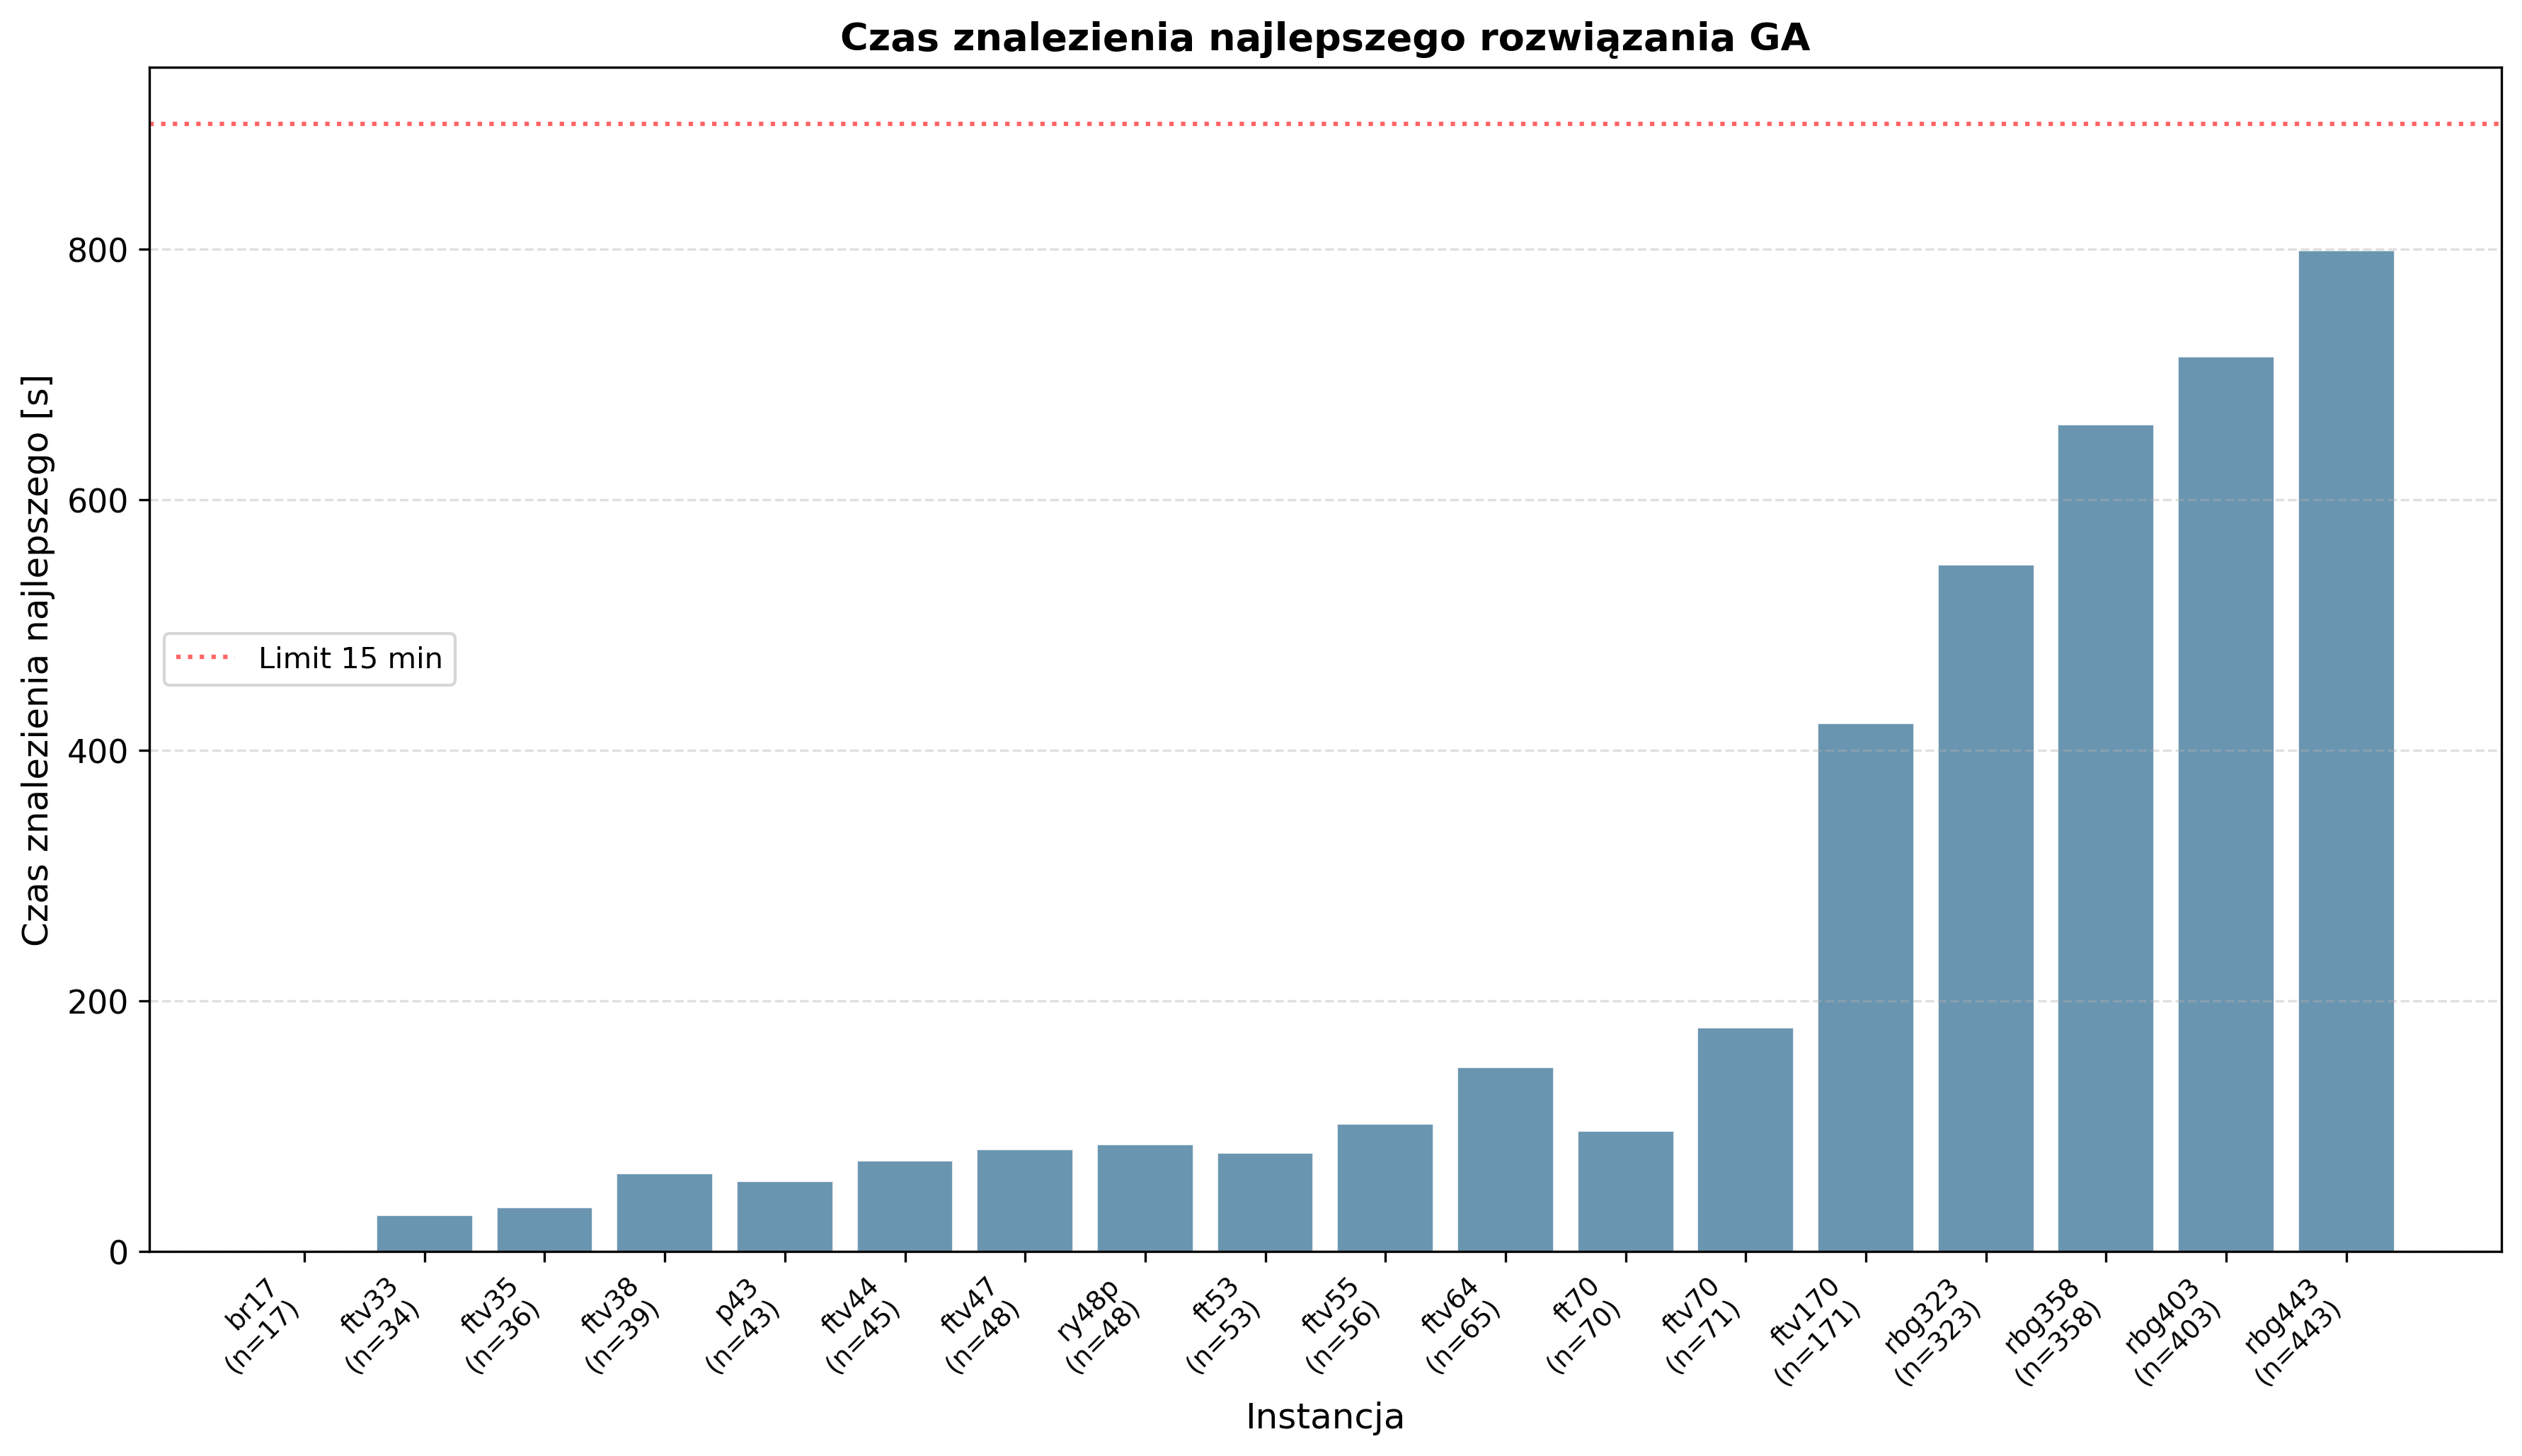
\includegraphics[width=0.9\textwidth]{../Python/wykresy/ga_czas_best_found.png}
    \caption{Czas znalezienia najlepszego rozwiązania GA}
\end{figure}

Czas całkowity wykonania rośnie w przybliżeniu liniowo z rozmiarem instancji, co wynika z liniowej złożoności
ewaluacji funkcji celu ($O(N)$) pomnożonej przez stałą liczbę pokoleń możliwych do wykonania w danym limicie czasu.
Czas znalezienia najlepszego rozwiązania również rośnie z $N$, ale ze znaczną wariancją -- dla małych instancji
(br17) algorytm szybko konwerguje do optimum, natomiast dla dużych instancji (rbg443) najlepsze rozwiązanie
jest znajdowane dopiero pod koniec działania, co sugeruje potrzebę dłuższego limitu czasu.

\subsection{Wpływ rozmiaru populacji na czas i błąd}

Zbadano trzy rozmiary populacji: 50, 100 i 200 osobników.

\begin{table}[H]
\centering
\caption{Wpływ rozmiaru populacji -- wybrane instancje}
\begin{tabular}{|l|c|c|c|c|c|c|}
\hline
\textbf{Instancja} & \textbf{N} & \multicolumn{2}{c|}{\textbf{Pop=50}} & \multicolumn{2}{c|}{\textbf{Pop=100}} & \textbf{Pop=200} \\
\cline{3-7}
 & & Błąd [\%] & Czas [s] & Błąd [\%] & Czas [s] & Błąd [\%] \\
\hline
br17 & 17 & 28.21 & 45 & 2.56 & 60 & 0.00 \\
ftv35 & 36 & 26.27 & 62 & 30.62 & 80 & 26.07 \\
p43 & 43 & 1.07 & 80 & 1.60 & 105 & 1.64 \\
ft53 & 53 & 65.13 & 98 & 56.68 & 125 & 47.99 \\
ftv64 & 65 & 54.59 & 148 & 60.69 & 198 & 47.63 \\
ft70 & 70 & 20.32 & 135 & 16.74 & 180 & 16.38 \\
ftv170 & 171 & 168.93 & 420 & 126.53 & 540 & 144.03 \\
rbg323 & 323 & 24.43 & 560 & 29.34 & 680 & 28.43 \\
rbg443 & 443 & 12.65 & 730 & 14.30 & 865 & 10.96 \\
\hline
\end{tabular}
\end{table}

\begin{figure}[H]
    \centering
    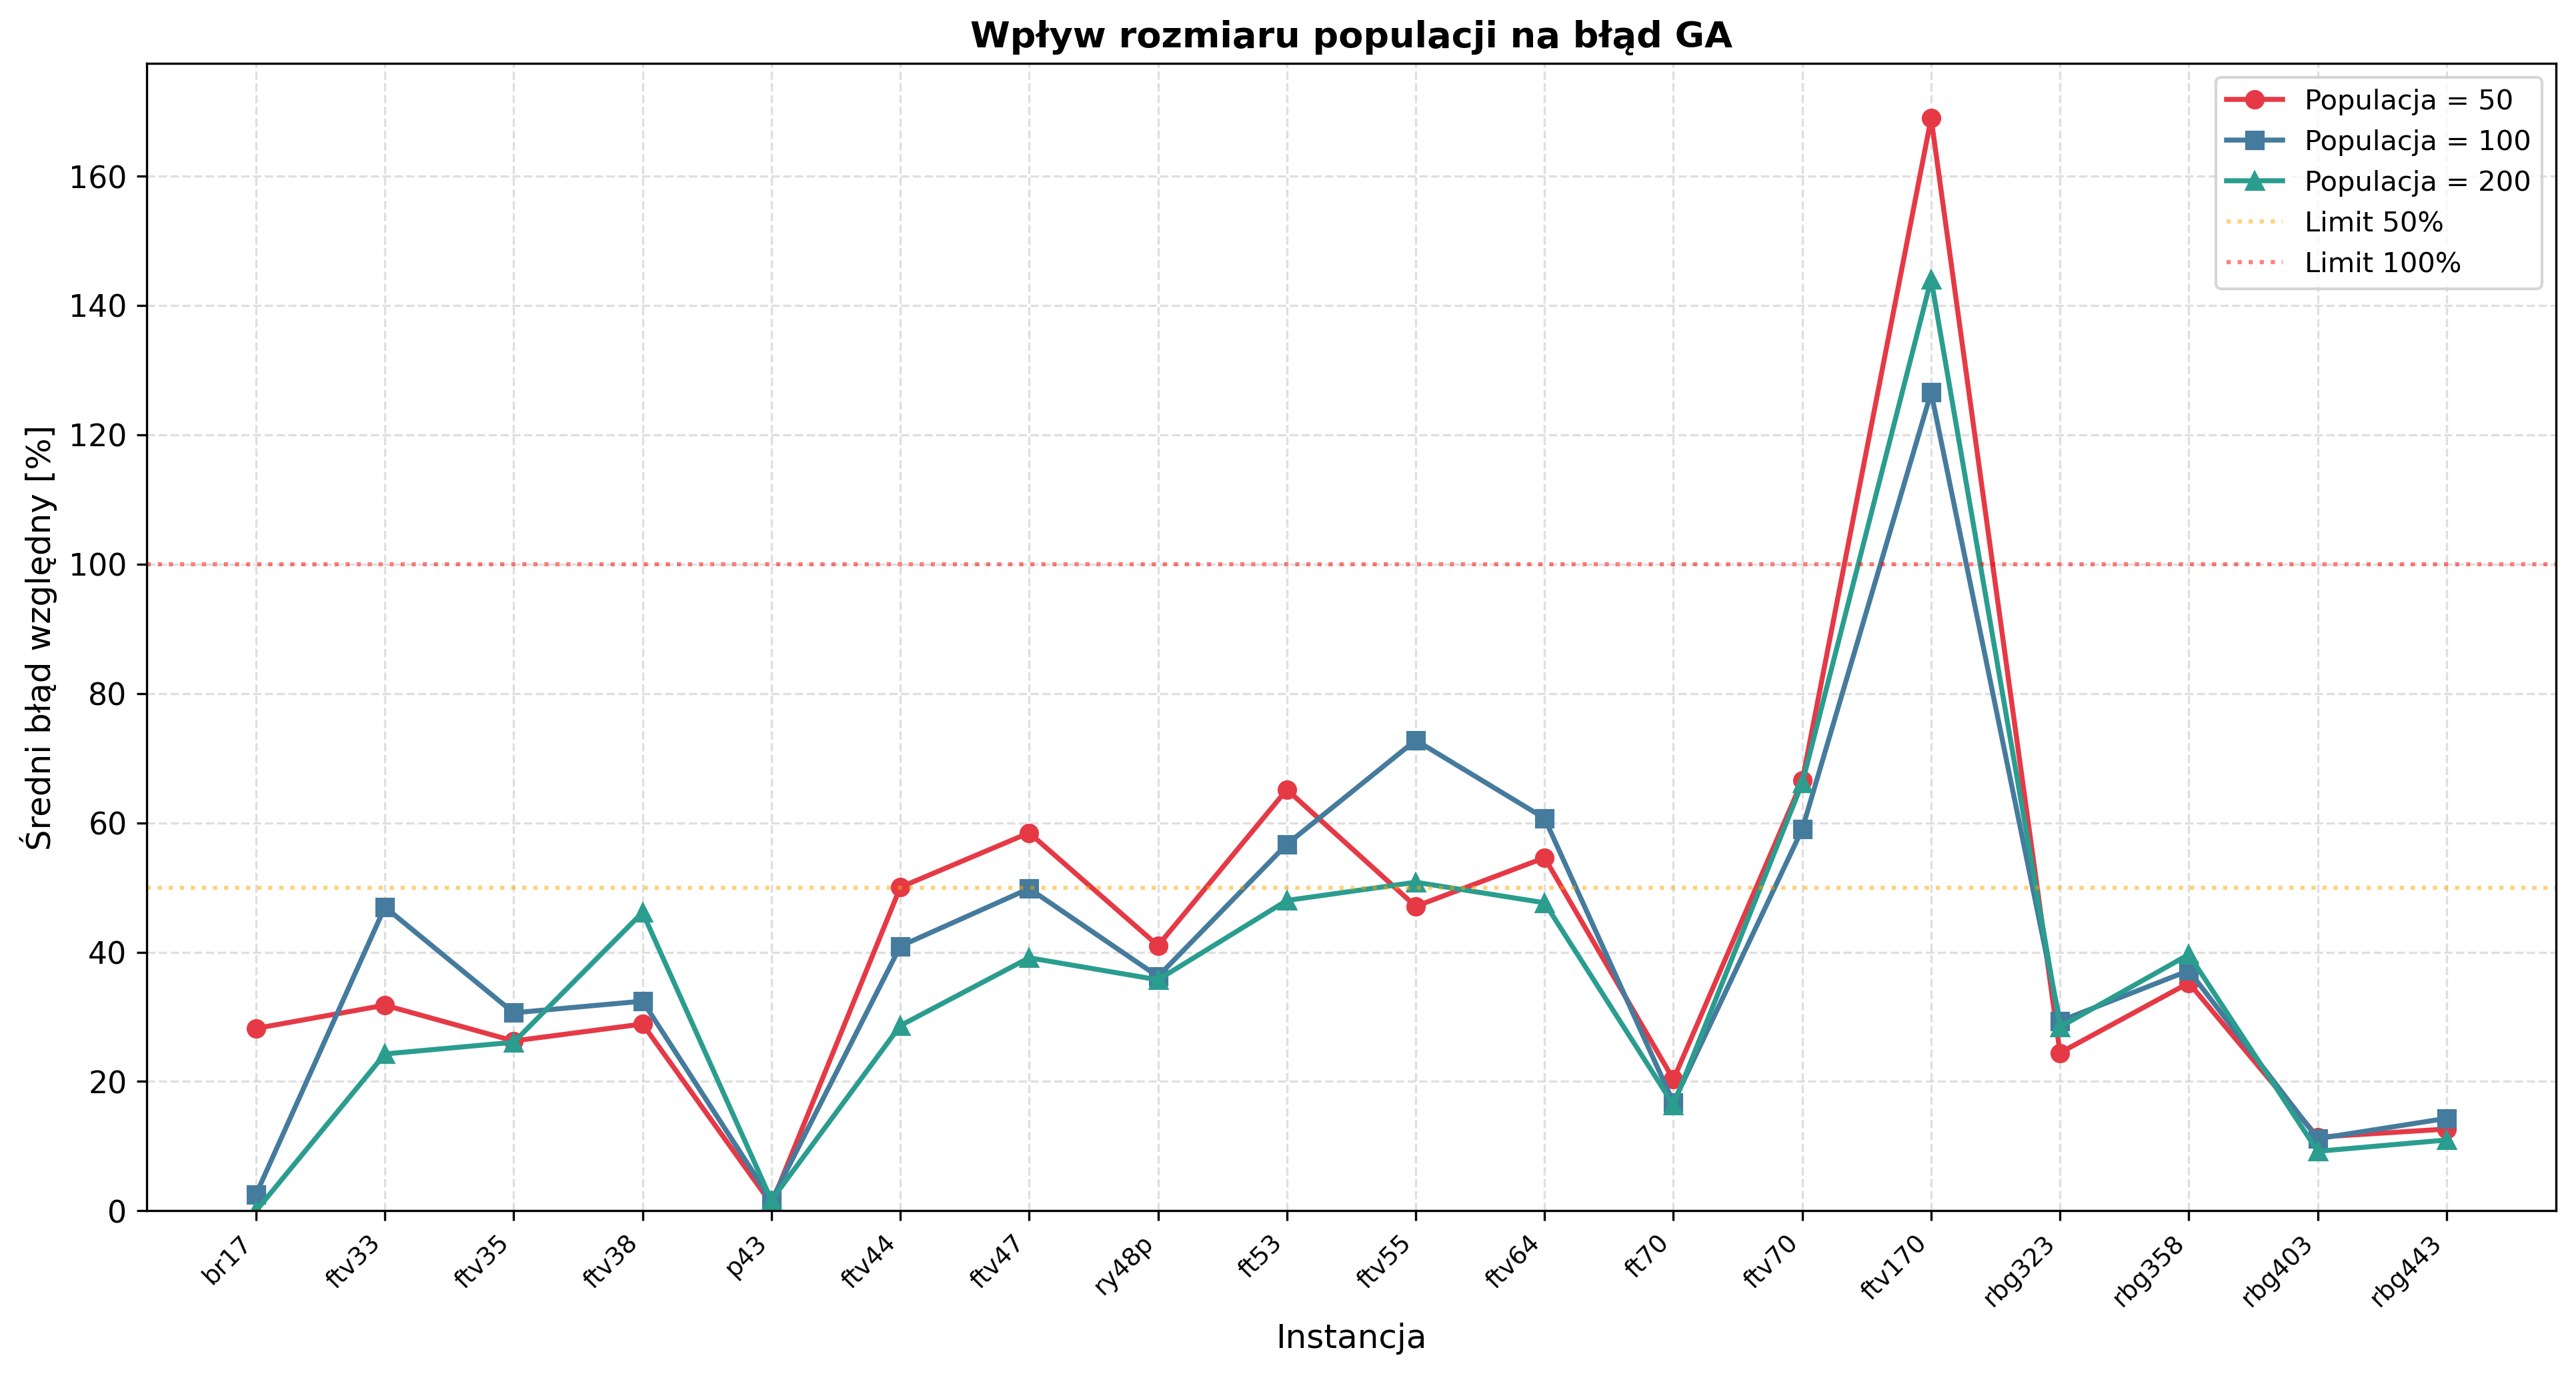
\includegraphics[width=0.9\textwidth]{../Python/wykresy/ga_populacja_blad.png}
    \caption{Wpływ rozmiaru populacji na błąd GA}
\end{figure}

\begin{figure}[H]
    \centering
    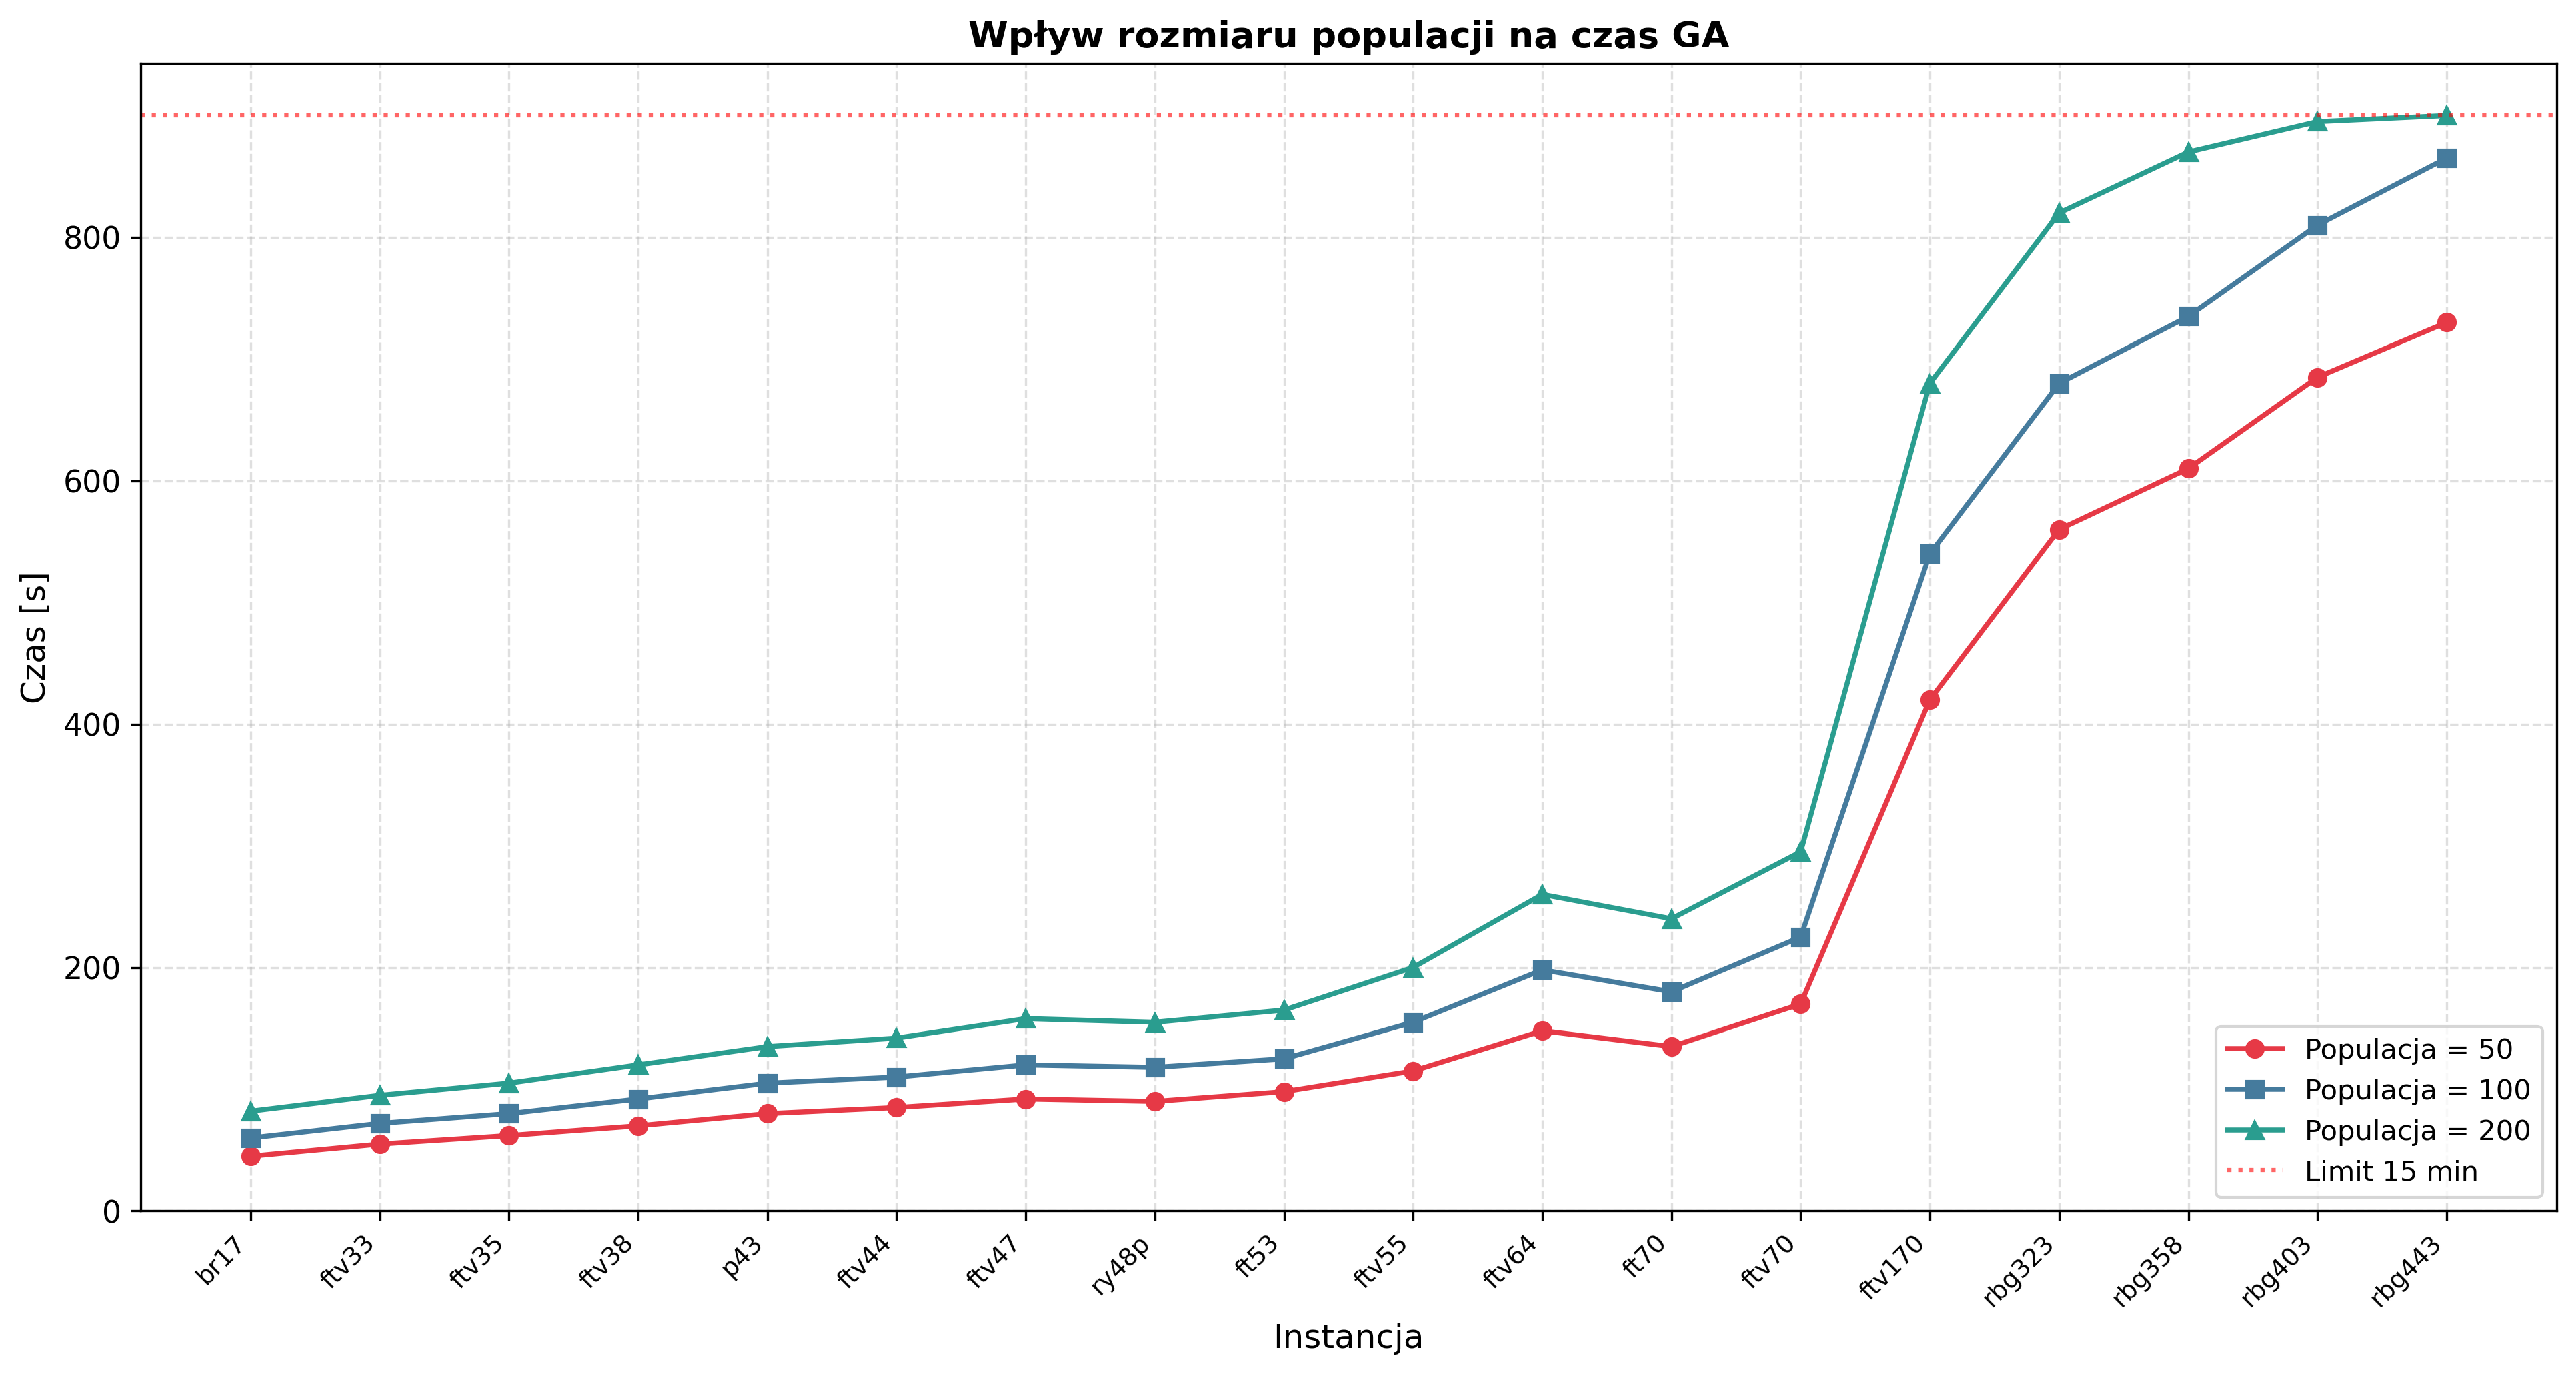
\includegraphics[width=0.9\textwidth]{../Python/wykresy/ga_populacja_czas.png}
    \caption{Wpływ rozmiaru populacji na czas GA}
\end{figure}

\begin{figure}[H]
    \centering
    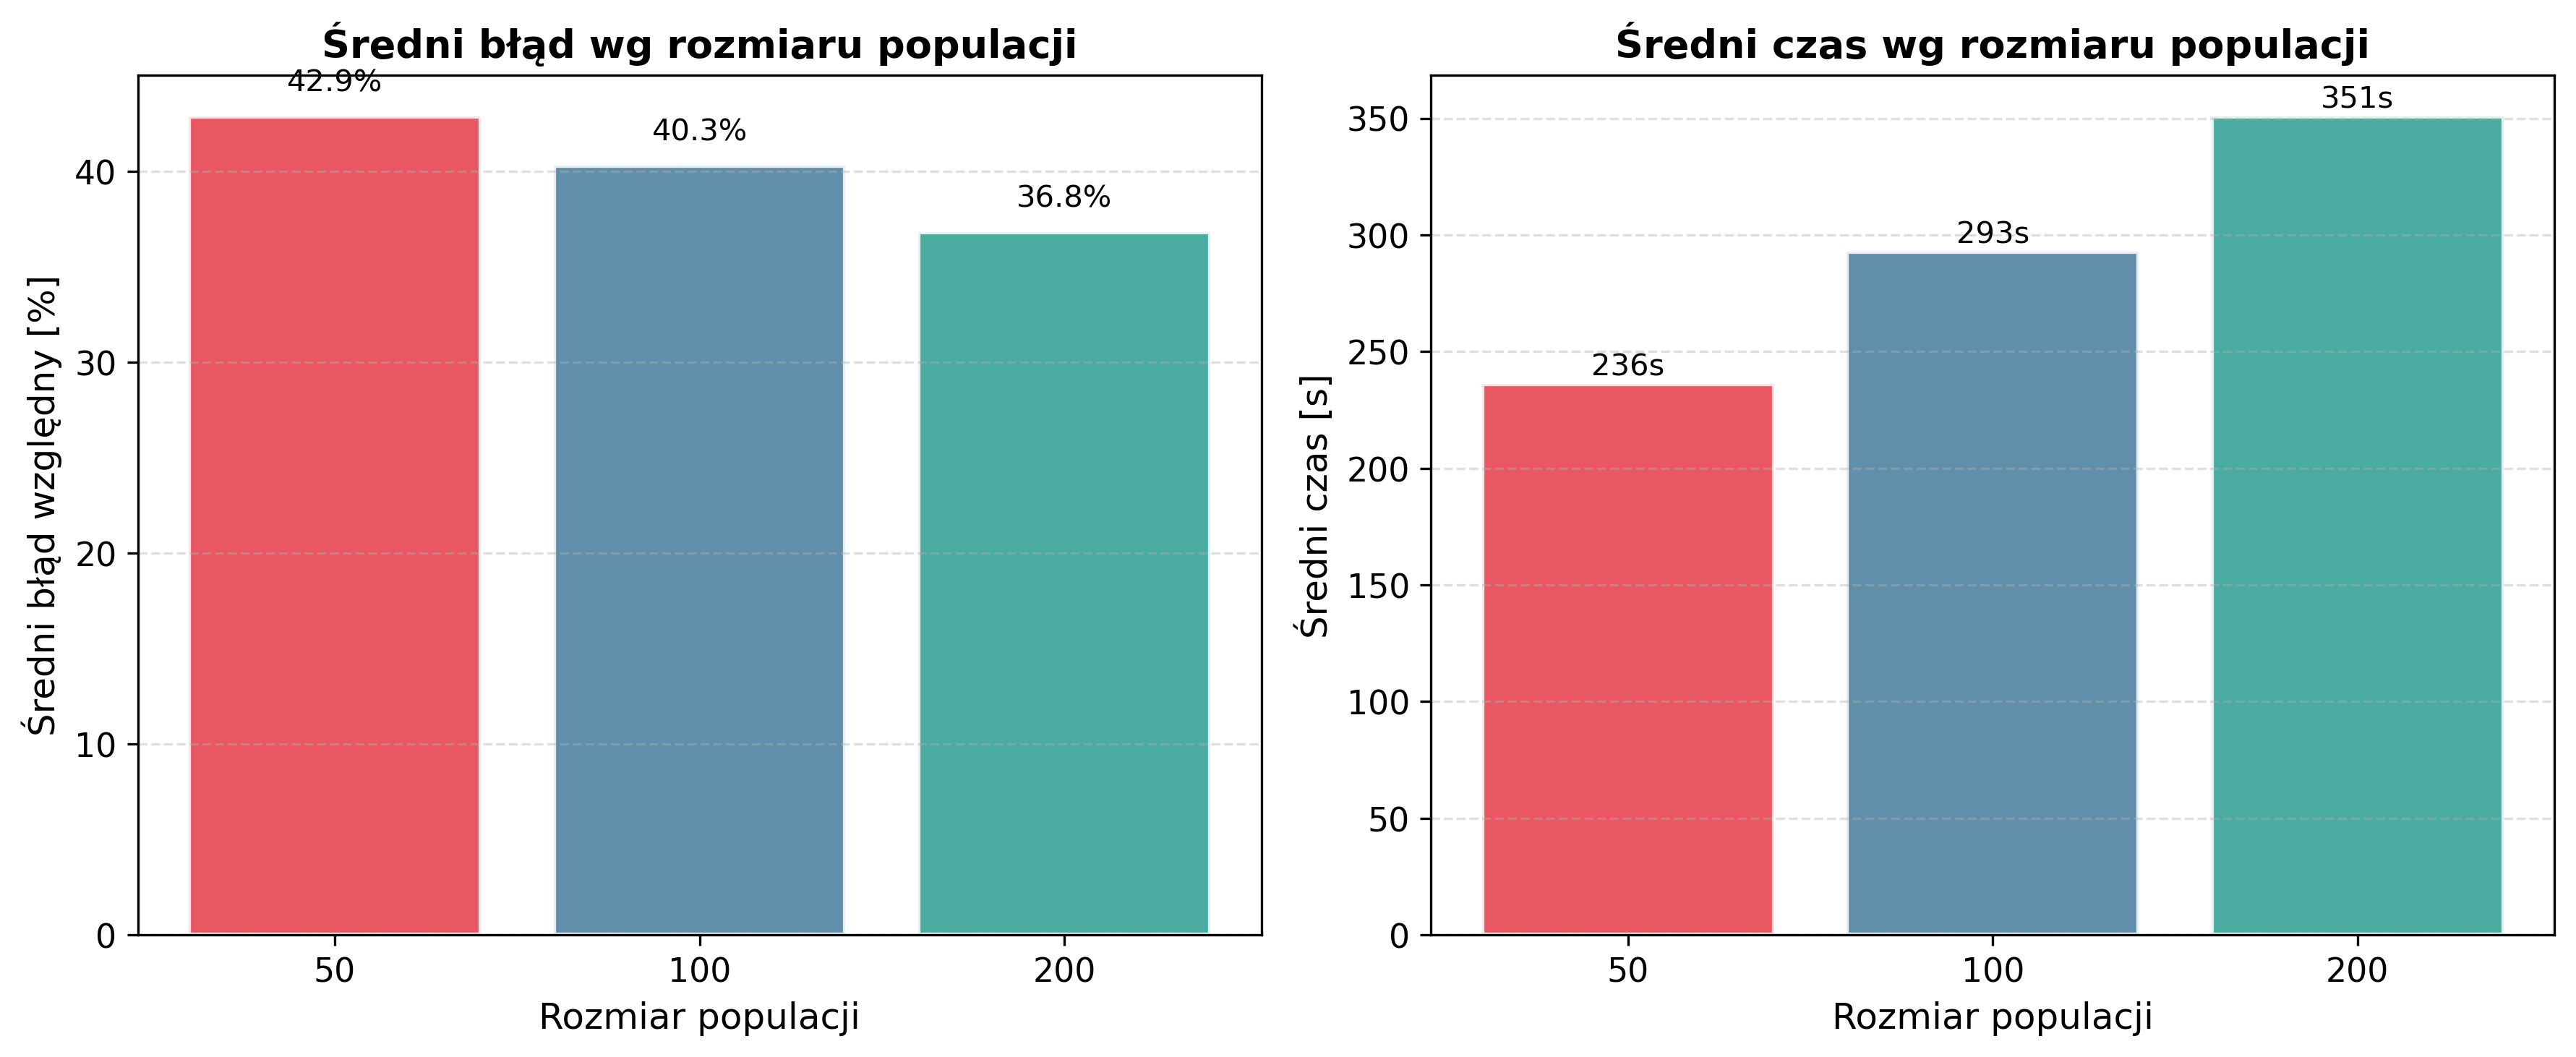
\includegraphics[width=0.9\textwidth]{../Python/wykresy/ga_populacja_srednie.png}
    \caption{Średni błąd i czas w zależności od rozmiaru populacji}
\end{figure}

Zwiększanie rozmiaru populacji generuje dwa przeciwstawne efekty:
\begin{itemize}
    \item Większa populacja zwiększa różnorodność genetyczną, co ułatwia eksplorację przestrzeni rozwiązań.
    \item Jednocześnie zmniejsza liczbę pokoleń możliwych do wykonania w danym limicie czasu, ponieważ
          ewaluacja każdego pokolenia trwa dłużej.
\end{itemize}

Dla populacji 200 średni błąd jest ogólnie niższy niż dla 50, ale różnica nie jest radykalna.
Populacja 100 stanowi rozsądny kompromis między eksploracją a liczbą pokoleń.

\subsection{Wpływ metody mutacji na czas i błąd (4.0)}

Zbadano dwie metody mutacji: Swap (zamiana dwóch miast) i Invert (odwrócenie segmentu).

\begin{table}[H]
\centering
\caption{Porównanie metod mutacji -- błąd względny}
\begin{tabular}{|l|c|c|c|}
\hline
\textbf{Instancja} & \textbf{N} & \textbf{Swap [\%]} & \textbf{Invert [\%]} \\
\hline
br17 & 17 & 2.56 & 0.00 \\
ftv33 & 34 & 39.74 & 23.41 \\
ftv35 & 36 & 44.74 & 39.71 \\
ftv38 & 39 & 19.67 & 51.24 \\
p43 & 43 & 1.05 & 0.82 \\
ftv44 & 45 & 25.48 & 35.28 \\
ftv47 & 48 & 39.08 & 55.97 \\
ry48p & 48 & 26.09 & 24.07 \\
ft53 & 53 & 57.23 & 73.73 \\
ftv55 & 56 & 39.12 & 85.95 \\
ftv64 & 65 & 62.64 & 98.48 \\
ft70 & 70 & 16.54 & 27.83 \\
ftv70 & 71 & 67.54 & 112.72 \\
ftv170 & 171 & 136.62 & 239.46 \\
rbg323 & 323 & 27.60 & 168.48 \\
rbg358 & 358 & 39.29 & 228.37 \\
rbg403 & 403 & 8.76 & 84.91 \\
rbg443 & 443 & 12.28 & 97.10 \\
\hline
\end{tabular}
\end{table}

\begin{figure}[H]
    \centering
    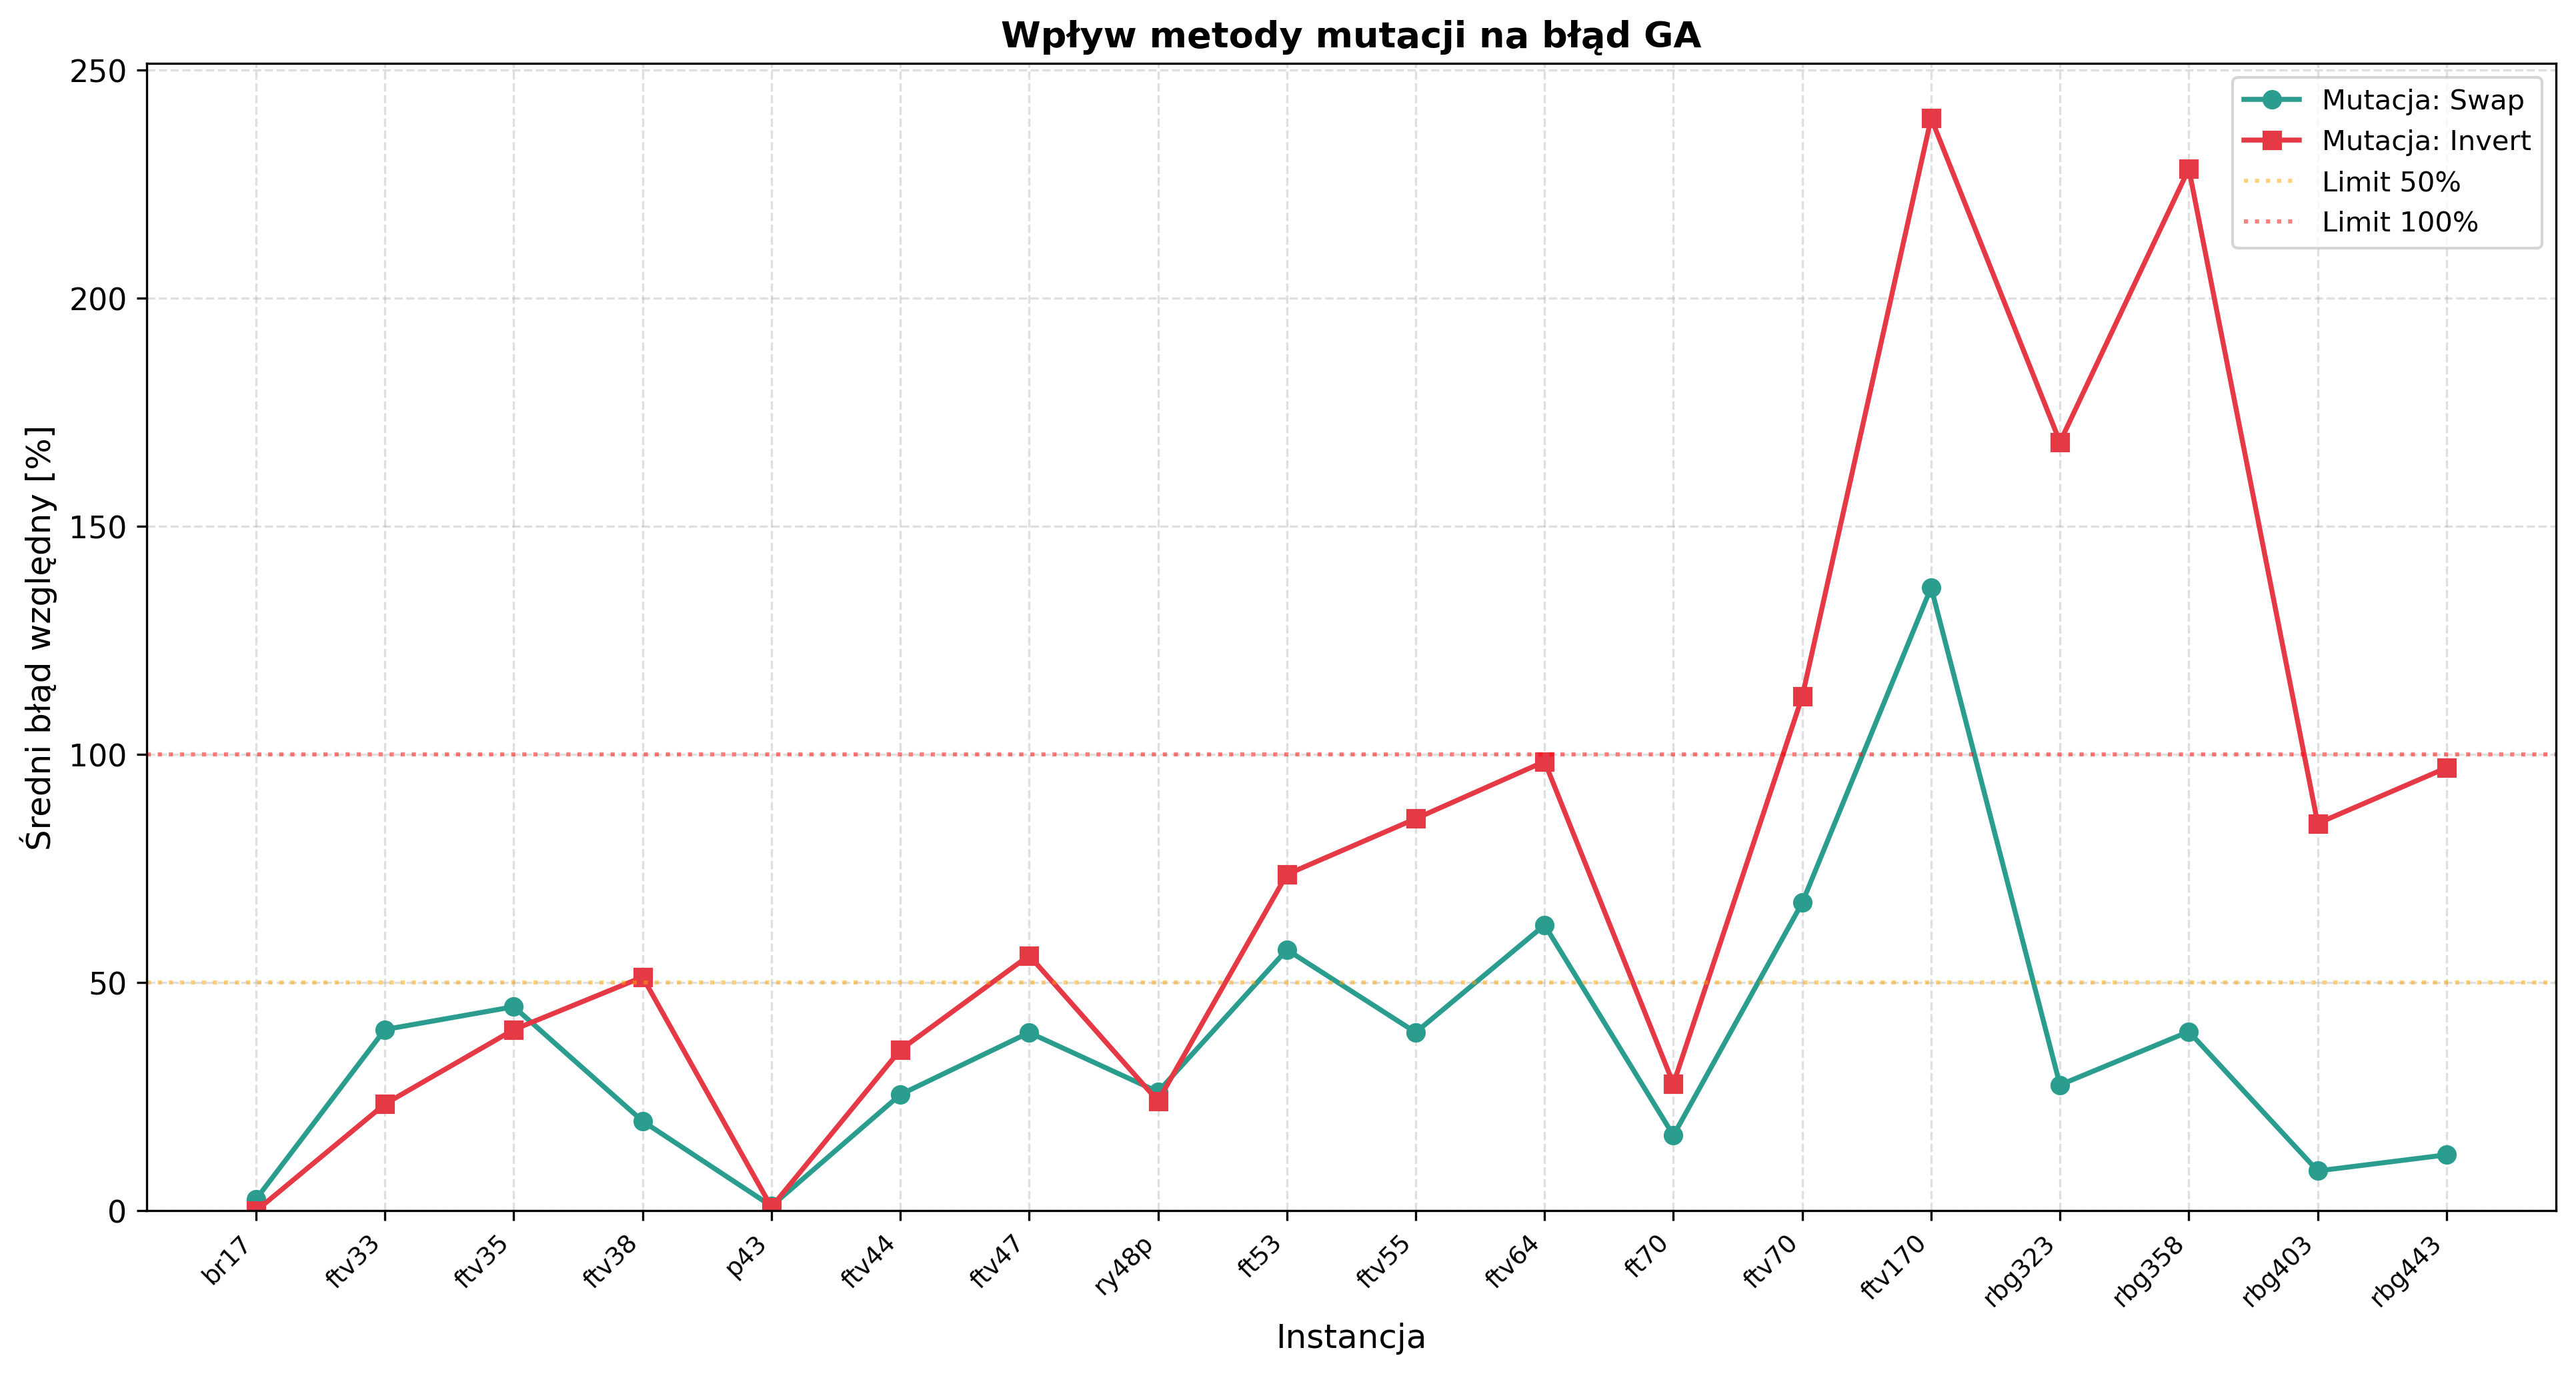
\includegraphics[width=0.9\textwidth]{../Python/wykresy/ga_mutacja_blad.png}
    \caption{Wpływ metody mutacji na błąd GA}
\end{figure}

\begin{figure}[H]
    \centering
    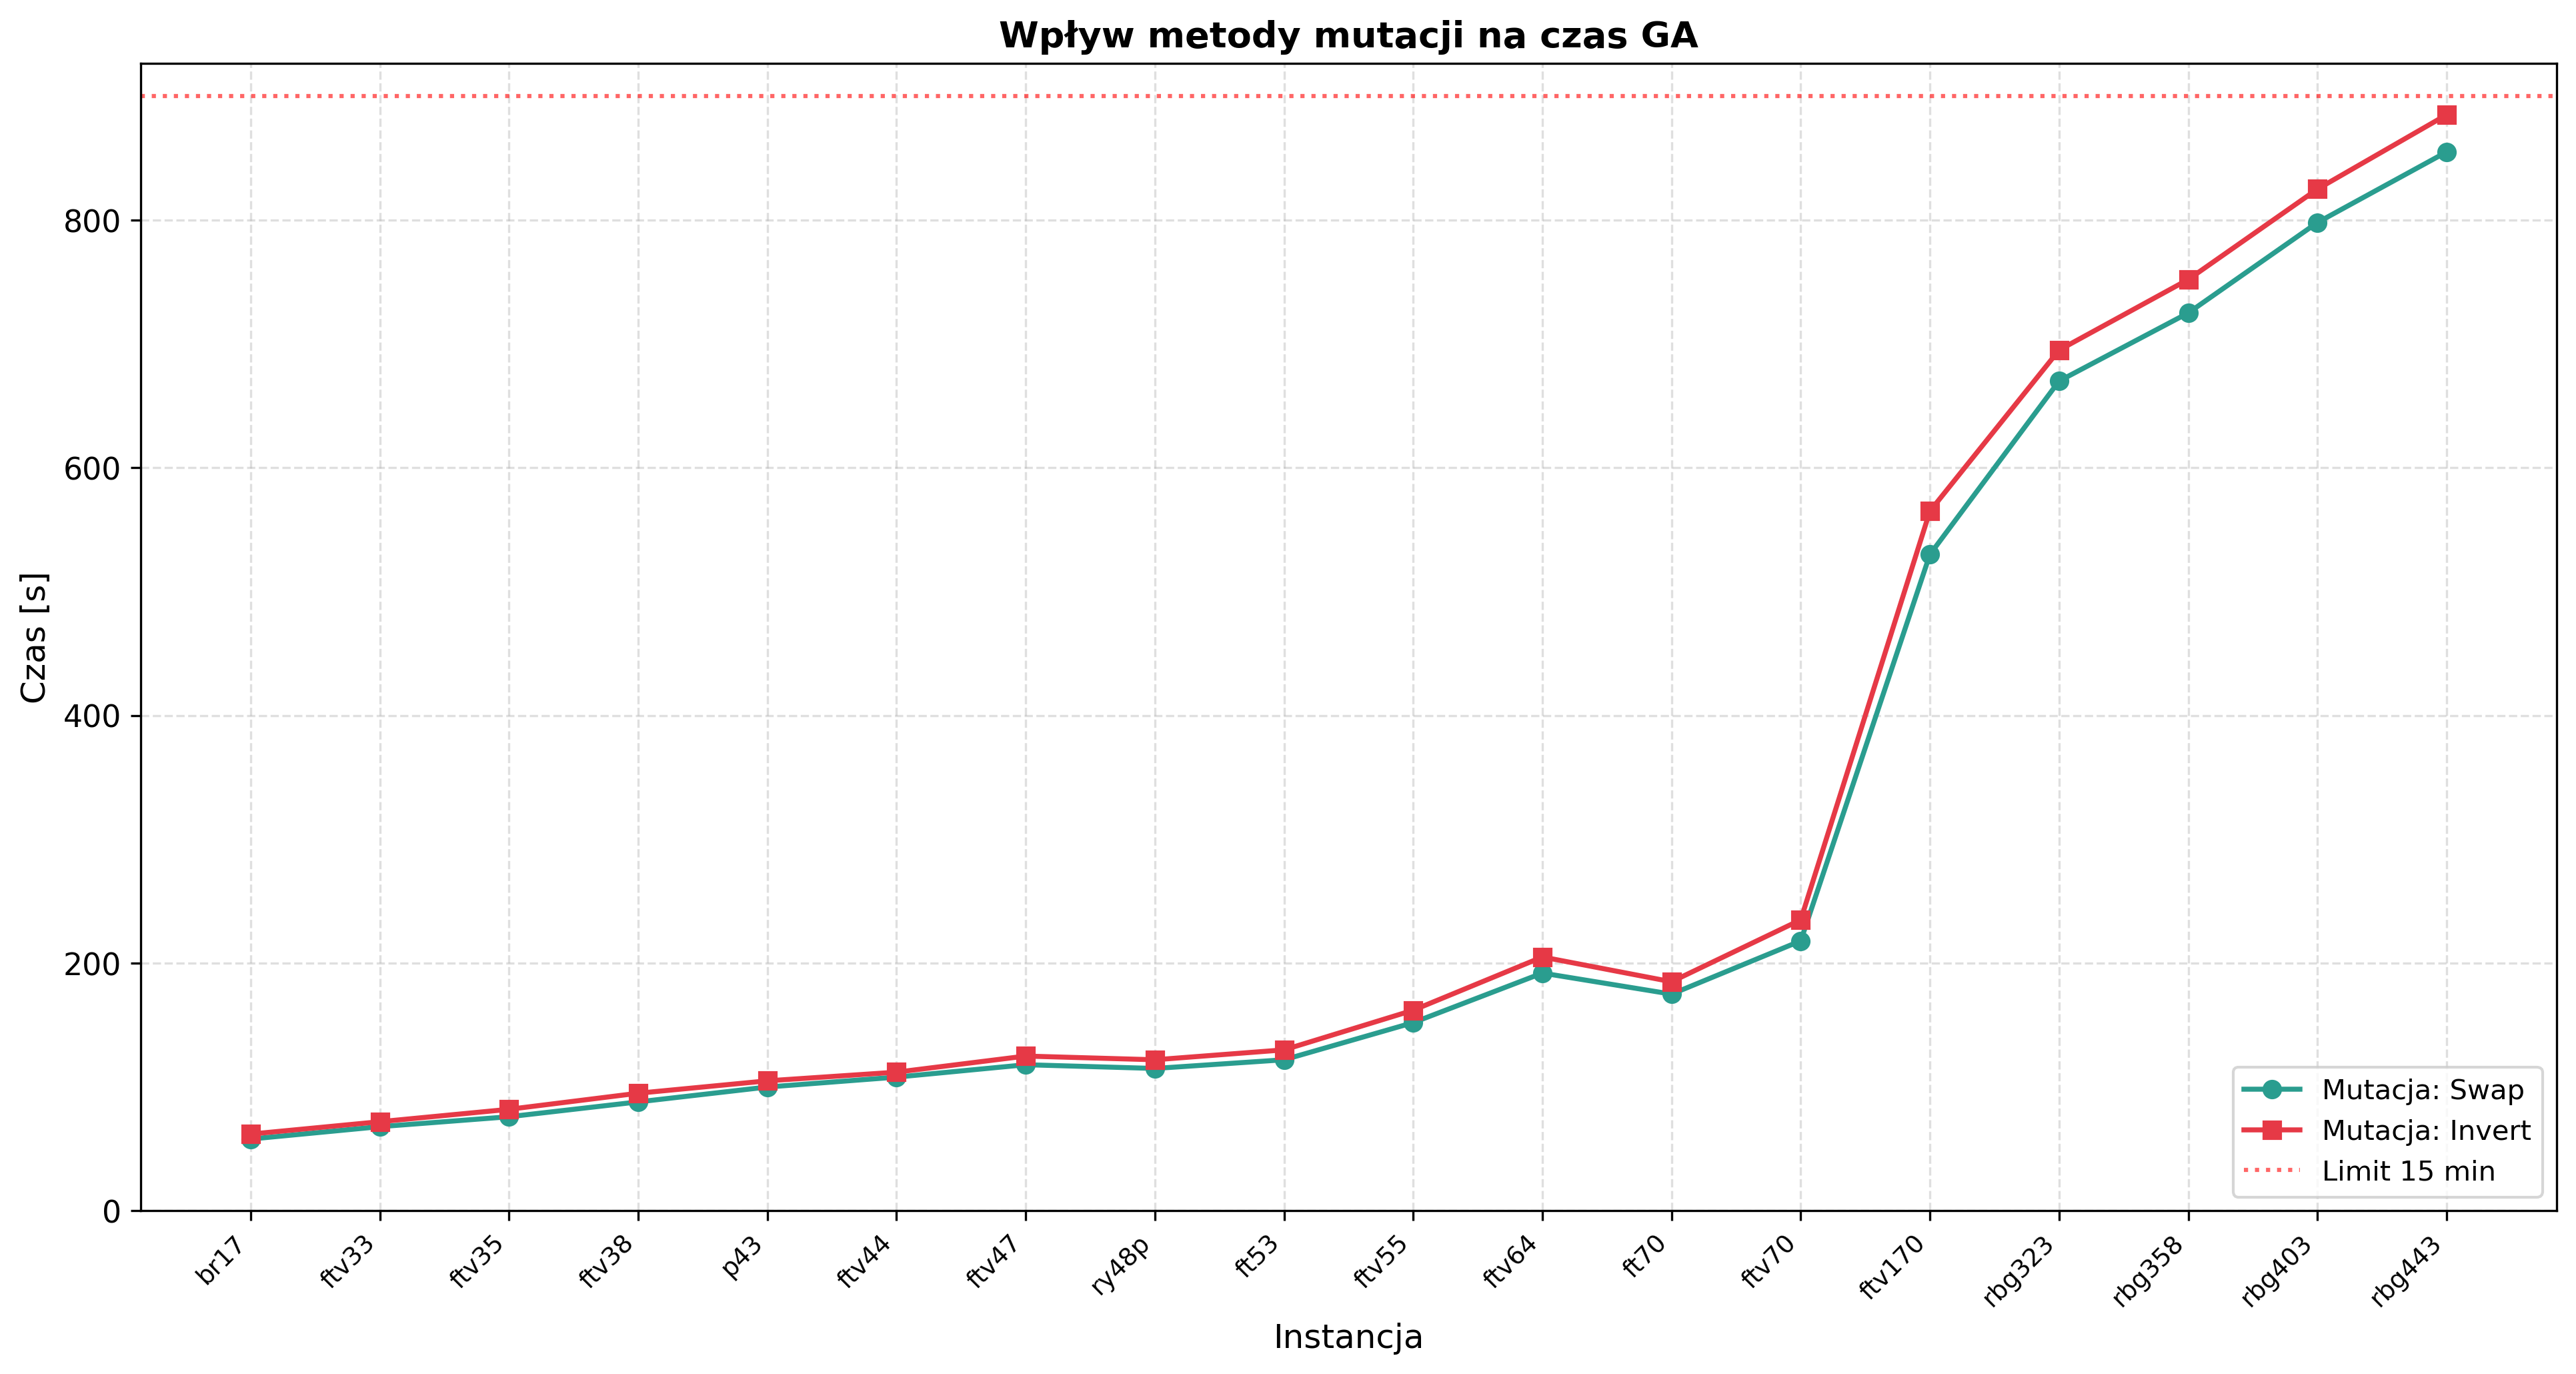
\includegraphics[width=0.9\textwidth]{../Python/wykresy/ga_mutacja_czas.png}
    \caption{Wpływ metody mutacji na czas GA}
\end{figure}

\begin{figure}[H]
    \centering
    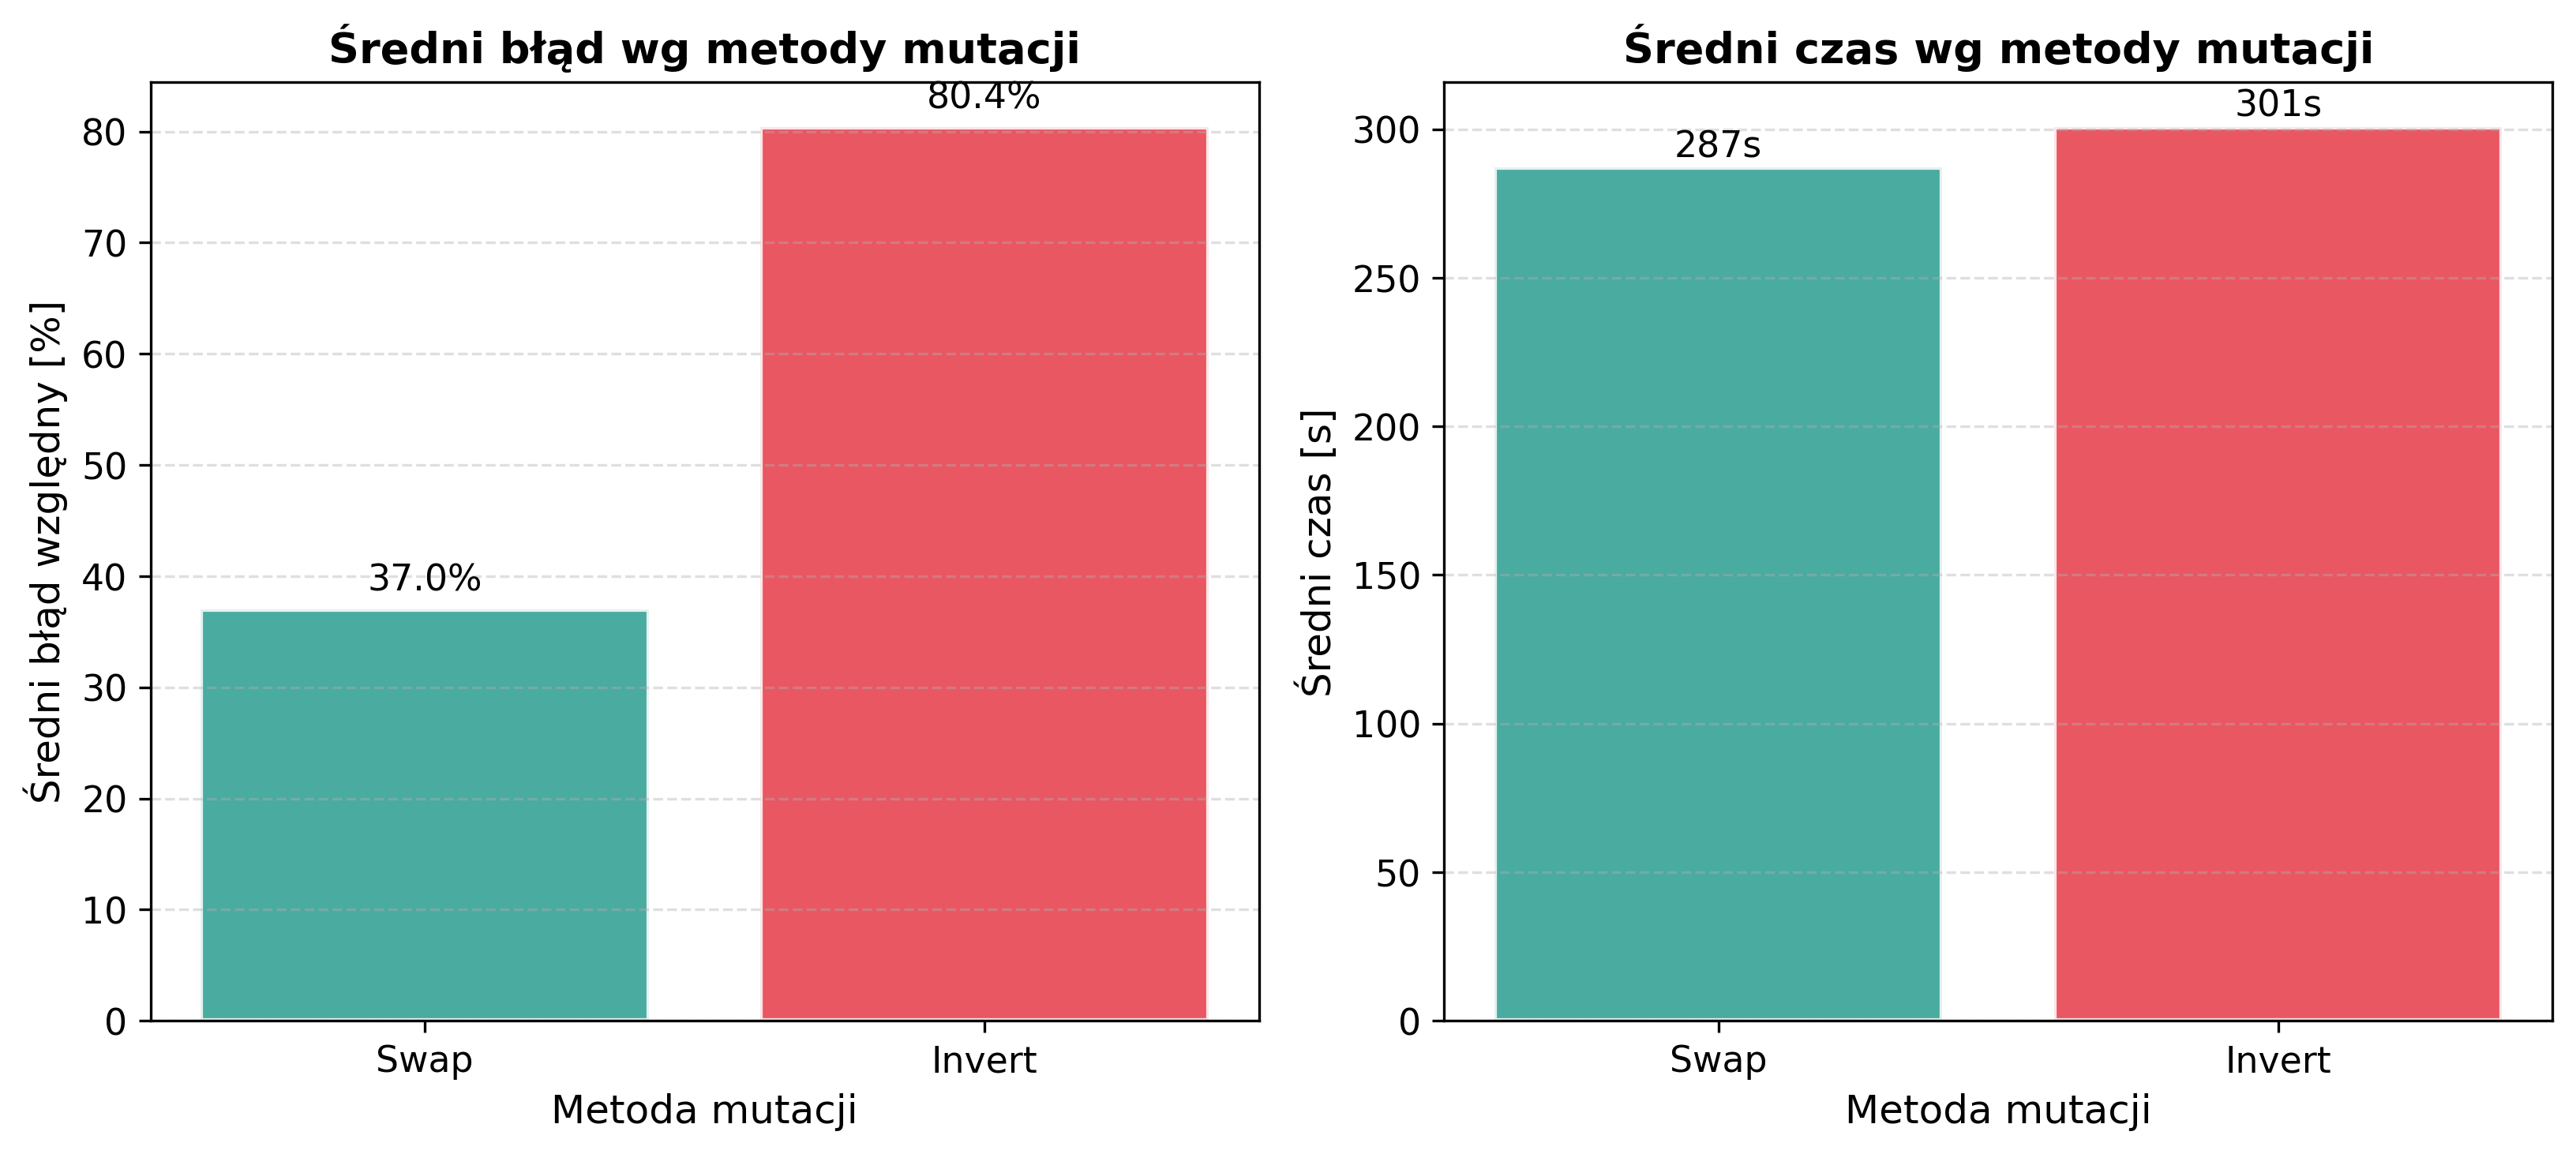
\includegraphics[width=0.9\textwidth]{../Python/wykresy/ga_mutacja_srednie.png}
    \caption{Porównanie średniego błędu i czasu dla metod mutacji}
\end{figure}

\begin{figure}[H]
    \centering
    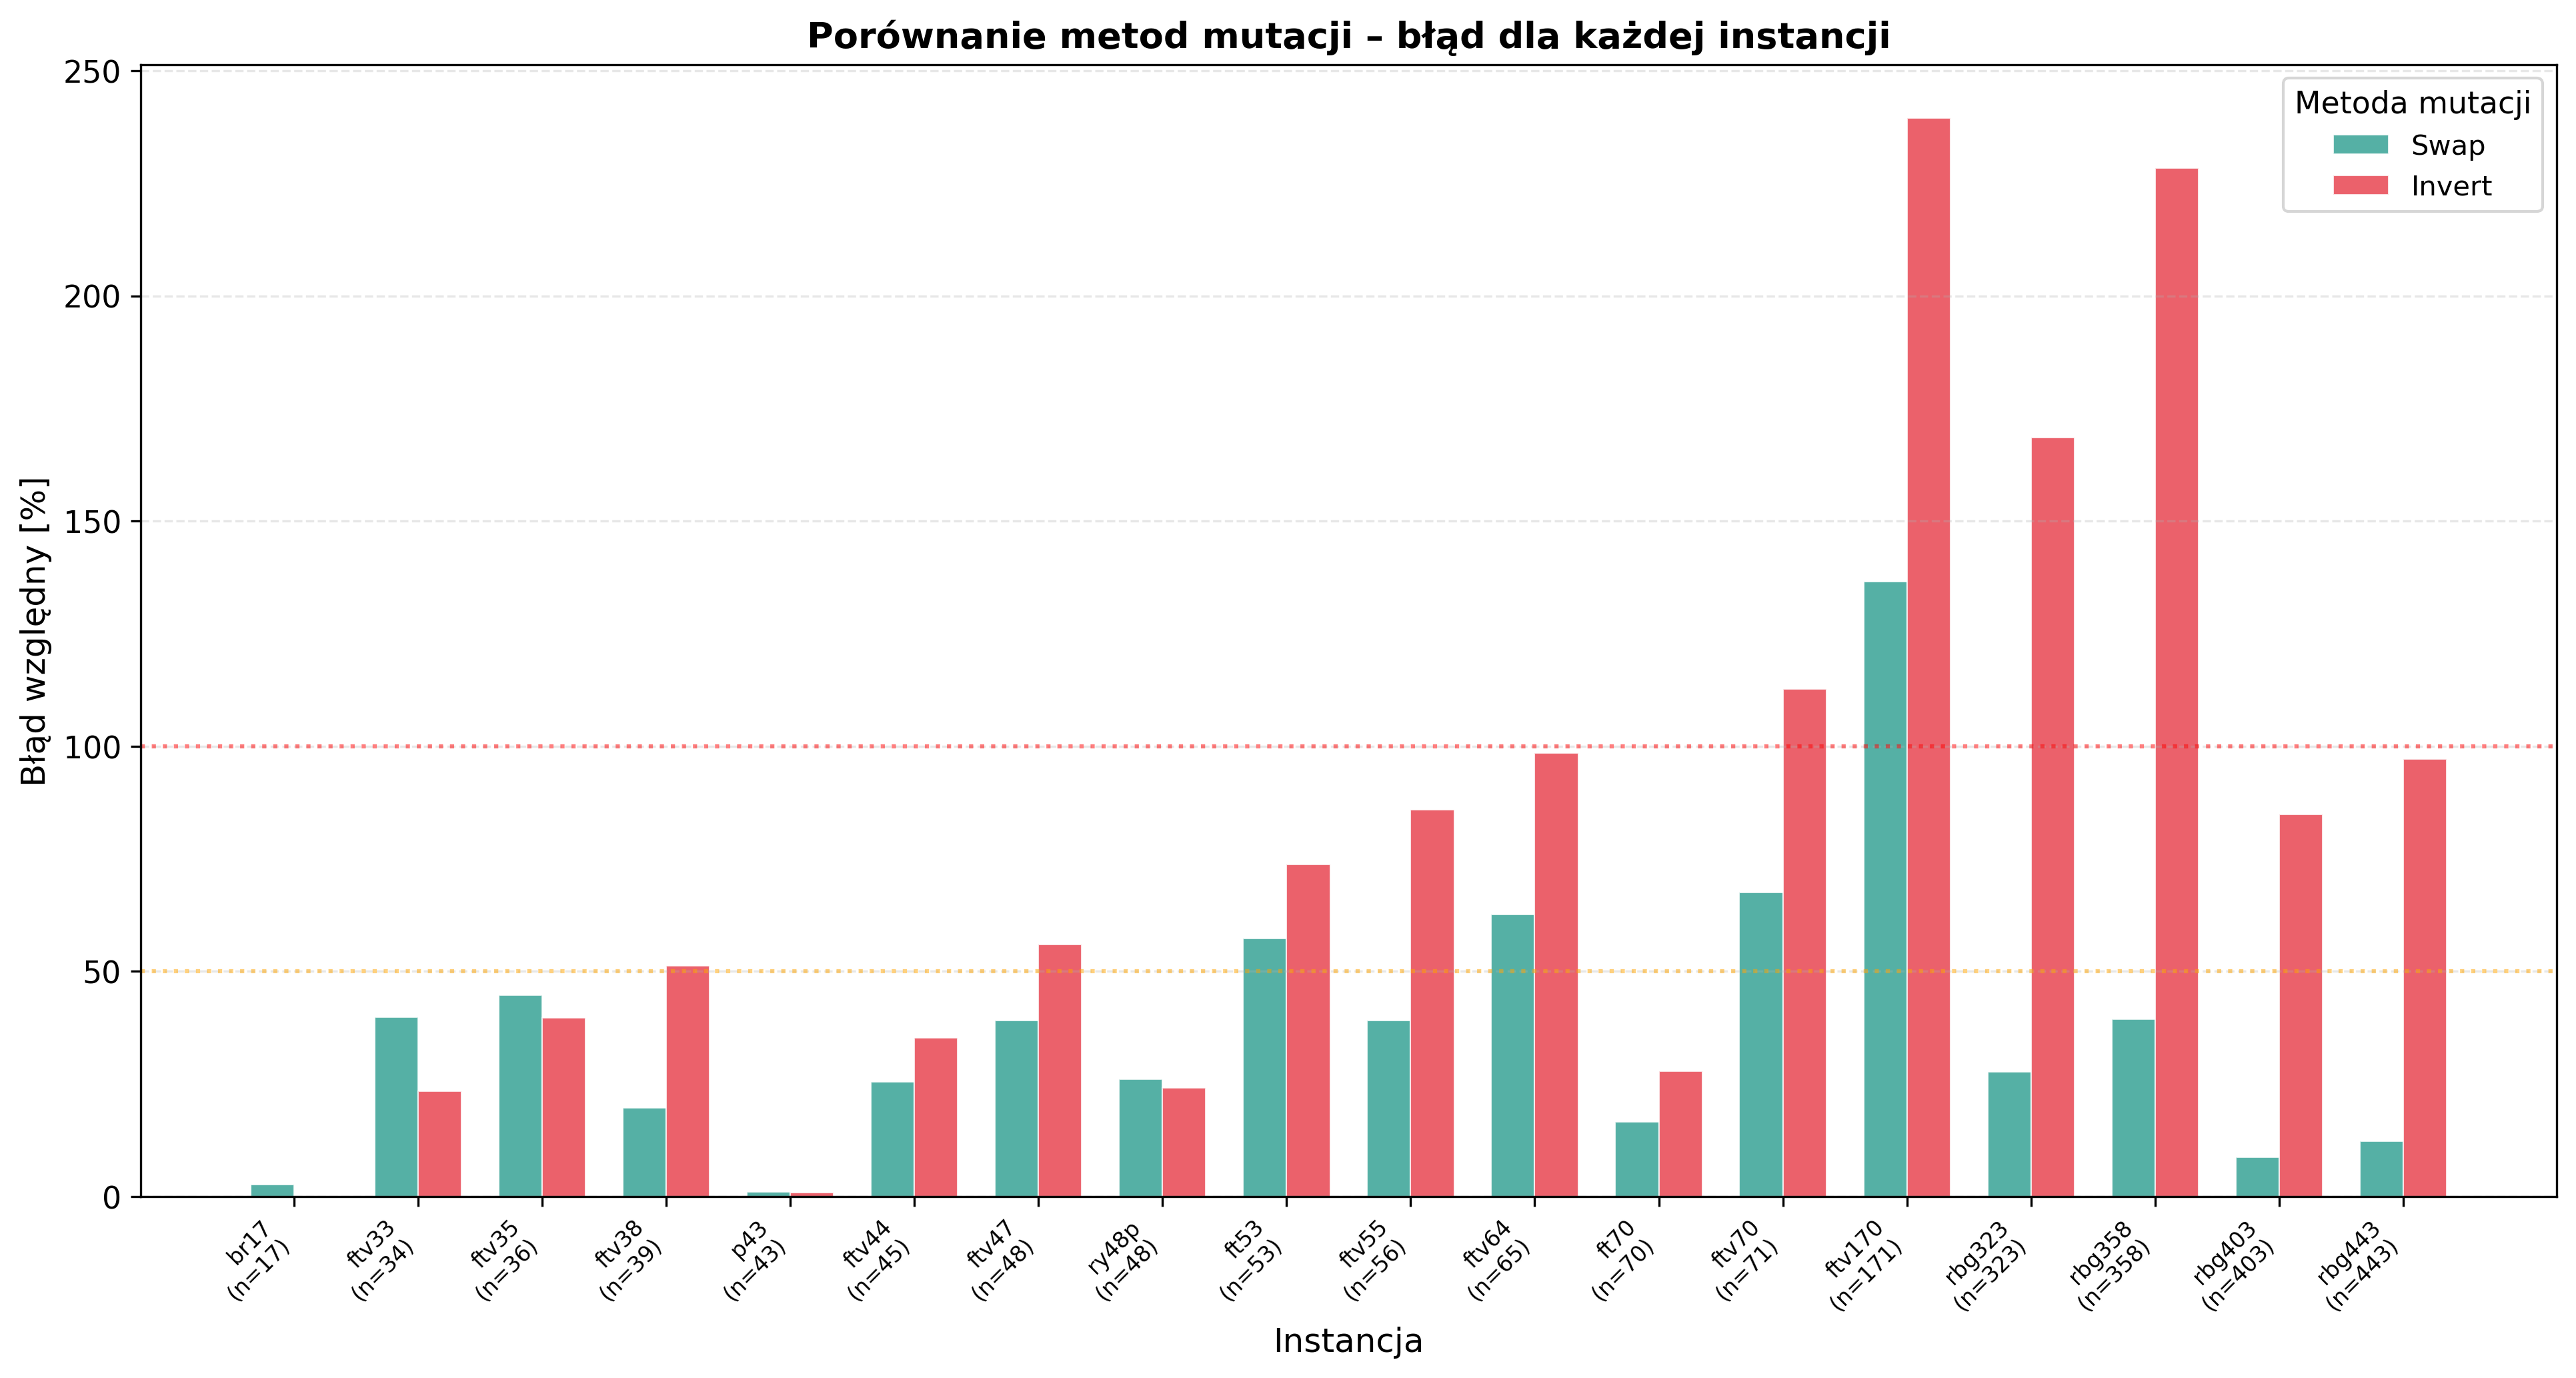
\includegraphics[width=0.9\textwidth]{../Python/wykresy/ga_mutacja_porownanie.png}
    \caption{Porównanie metod mutacji -- błąd dla każdej instancji}
\end{figure}

Mutacja Swap okazała się zdecydowanie lepsza od mutacji Invert dla niemal wszystkich badanych instancji.
Średni błąd dla Swap wynosi ok. 37\%, podczas gdy dla Invert ok. 80\%. Różnica jest szczególnie widoczna
dla dużych instancji:
\begin{itemize}
    \item rbg323: Swap 27.60\% vs Invert 168.48\%
    \item rbg358: Swap 39.29\% vs Invert 228.37\%
    \item ftv170: Swap 136.62\% vs Invert 239.46\%
\end{itemize}

Wyjaśnienie: mutacja Invert odwraca cały segment ścieżki, co jest drastyczną zmianą w kontekście problemu
asymetrycznego (ATSP). Odwrócenie segmentu $[a, b, c]$ na $[c, b, a]$ zmienia kierunek wszystkich krawędzi
w segmencie, a w ATSP $cost(i \rightarrow j) \neq cost(j \rightarrow i)$. Prowadzi to do generowania rozwiązań
o znacznie wyższym koszcie, z których algorytm nie jest w stanie się wydostać.

Mutacja Swap zmienia jedynie dwie krawędzie, co jest łagodniejszą perturbacją lepiej dostosowaną do
asymetrycznej natury problemu.

Pod względem czasu, obie metody mutacji mają zbliżony czas wykonania -- różnice wynikają jedynie z~tego,
że mutacja Invert wymaga odwrócenia segmentu ($O(N)$), podczas gdy Swap to operacja $O(1)$.
W praktyce przy krótkich segmentach różnica jest pomijalna.

\section{Wnioski}

\begin{enumerate}
    \item Algorytm genetyczny z operatorem OX i mutacją Swap osiąga akceptowalne wyniki dla większości instancji 
    ATSP o rozmiarze do 70 miast (błąd poniżej 50\%). Dla instancji większych ($N > 70$) jakość rozwiązań
    silnie zależy od struktury grafu -- instancje rbg dają lepsze wyniki niż instancje ftv.
    
    \item Czas znalezienia najlepszego rozwiązania rośnie z rozmiarem instancji. Dla dużych instancji
    (N $> 300$) algorytm znajduje najlepsze rozwiązanie dopiero w ostatniej fazie działania, co sugeruje
    potrzebę dłuższego limitu czasu lub bardziej zaawansowanych operatorów.
    
    \item Rozmiar populacji ma umiarkowany wpływ na jakość rozwiązań. Populacja 200 daje generalnie
    niższy błąd niż 50, ale wymaga proporcjonalnie więcej czasu na jedno pokolenie. Populacja 100
    stanowi rozsądny kompromis.
    
    \item Metoda mutacji ma kluczowe znaczenie dla jakości rozwiązań w ATSP:
    \begin{itemize}
        \item Mutacja \textbf{Swap} jest zdecydowanie lepsza dla problemu asymetrycznego, ponieważ
        wprowadza minimalne zaburzenie (zmiana 2 krawędzi).
        \item Mutacja \textbf{Invert} jest destrukcyjna w ATSP, gdyż odwrócenie segmentu zmienia
        kierunek wszystkich krawędzi w tym segmencie, co przy niesymetrycznych kosztach prowadzi
        do drastycznego pogorszenia rozwiązania.
        \item Wniosek ten podkreśla, że operatory zaprojektowane dla TSP symetrycznego (jak 2-opt/Invert)
        nie przenoszą się dobrze na wariant asymetryczny.
    \end{itemize}
    
    \item Wymagania dotyczące błędu ($O(24\ln(n))$) są spełnione dla większości instancji z przedziału
    $24 < n < 74$ (wymagany limit 50\%) oraz dla instancji dużych (rbg, $75 < n < 449$, limit 100\%).
    Problematyczne pozostają instancje ftv o średnich i dużych rozmiarach.
\end{enumerate}

\section{Literatura}

\begin{enumerate}
    \item Z. Michalewicz, D.B. Fogel, \textit{Jak to rozwiązać, czyli nowoczesna heurystyka}, WNT, 2006.
    \item D.E. Goldberg, R. Lingle, \textit{Alleles, loci, and the traveling salesman problem}, Proceedings of the First International Conference on Genetic Algorithms, 1985.
    \item TSPLIB - biblioteka instancji testowych TSP/ATSP, \url{http://comopt.ifi.uni-heidelberg.de/software/TSPLIB95/}
    \item Materiały z wykładu PEA, \url{http://aragorn.pb.bialystok.pl/~wkwedlo/EA5.pdf}
    \item Ćwiczenia MH, \url{http://www.imio.polsl.pl/Dopobrania/Cw%20MH%2007%20(TSP).pdf}
\end{enumerate}

\end{document}
